%!TEX program = xelatex
%!TEX root = ../all.tex

\chapter{Multilayer networks}


So far, we have only considered models in which there is a \emph{single} set of parameters to be learned and these parameters act \emph{directly} on the input. A typical example is a generalized linear model (GLM), whose functional form can be written as
\begin{myequation}
y(\x)=f(\w^{T}\x+b),
\end{myequation}
where $\w$ and $b$ are learned from data and the nonlinearity $f$ is fixed in advance. The key feature of this class of models is that the input $\x$ is transformed in one step into a scalar (or a small vector) through a linear combination, and then possibly passed through a simple nonlinearity. This is a powerful and interpretable framework, but it is also fundamentally limited: the hypothesis class only contains functions that are ``almost linear'' in the input, with the departure from linearity determined entirely by the fixed choice of $f$.

A much richer class of models is obtained if we allow the prediction to be computed through a \emph{sequence} of transformations. Conceptually, instead of applying a single transformation to $\x$, we apply many, one after another, and we let intermediate representations be produced and then re-used. This naturally leads to \emph{networks} of functions arranged in \emph{layers}. In this perspective, a multilayer model is not just a single GLM, but a composition of several GLM-like blocks, each block producing a new representation that becomes the input to the next one. The depth of the network, that is, the number of such composed blocks, is one of the most important architectural choices one makes when designing a neural model.

To build intuition, it is useful to view even standard linear and logistic regression as extremely shallow networks, where the ``network'' contains essentially one affine map $\x \mapsto \w^T \x + b$ followed (or not) by a fixed nonlinearity.

\begin{center}
\begin{tikzpicture}
\begin{scope}[scale=1]
     \Vertex[Math, x=1,y=0, color=xkcdFadedBlue, opacity=.8, shape = rectangle, label = \x, fontsize=\footnotesize, style={minimum width=1.4cm, minimum height=3mm, line width=.1pt}]{B0}
     \Text[position=below,x=1,y=0, distance=1.2mm, fontsize=\scriptsize]{$d$}
     \Vertex[Math, x=2.25,y=0, color=xkcdTurquoise, opacity=.5, shape = rectangle, label = \w, fontsize=\footnotesize, style={minimum width=.3cm, minimum height=1.4cm, line width=1pt,  draw=xkcdReddish}]{B1}
     \Text[position=right,x=2.25,y=.5, distance=2mm, fontsize=\scriptsize]{$d$}
     \Edge[lw=.5pt, Direct](B0)(B1)
     \Vertex[Math, x=3,y=0, color=xkcdFadedBlue, opacity=.5, shape = rectangle, fontsize=\footnotesize, style={minimum width=3mm, minimum height=3mm, line width=.1pt}]{B2}
     \Edge[lw=.5pt, Direct](B1)(B2)
     \Vertex[Math, x=4,y=0, color=xkcdLightGrey, label = +, size = .4, opacity=.5, fontsize=\footnotesize, style={line width=.5pt}]{C}
     \Edge[lw=.5pt, Direct](B2)(C)
     \Vertex[Math, x=4,y=-1, color=xkcdTurquoise, label = b, opacity=.5, shape = rectangle, fontsize=\footnotesize, style={minimum width=3mm, minimum height=3mm, line width=1pt,  draw=xkcdReddish}]{B3}
    \Edge[lw=.5pt, Direct](B3)(C)
    \Vertex[Math, x=5,y=0, color=xkcdLipstickRed, opacity=.5, shape = rectangle, fontsize=\footnotesize, style={minimum width=3mm, minimum height=3mm, line width=.1pt}]{C3}
    \Edge[lw=.5pt, Direct](C)(C3)
    \Text[x=-3,y=0, fontsize=\footnotesize]{Linear regression}
\end{scope}
\end{tikzpicture}
\end{center}

In linear regression, the last block simply outputs the affine response; equivalently, we may interpret $\varphi$ as the identity map. The model has no nonlinearity whatsoever, which makes it fast and interpretable but limits its expressiveness to the class of affine functions of the input. Logistic regression takes one further step: it adds an additional fixed nonlinearity, typically the sigmoid, whose role is to map real-valued scores to probabilities in $(0,1)$, thus making the output suitable for binary classification.

\begin{center}
\begin{tikzpicture}
 \begin{scope}[scale=1]
  \Vertex[Math, x=1,y=0, color=xkcdFadedBlue, opacity=.8, shape = rectangle, label = \x, fontsize=\footnotesize, style={minimum width=1.4cm, minimum height=3mm, line width=.1pt}]{B0}
 \Text[position=below,x=1,y=0, distance=1.2mm, fontsize=\scriptsize]{$d$}
 \Vertex[Math, x=2.25,y=0, color=xkcdTurquoise, opacity=.5, shape = rectangle, label =\w, fontsize=\footnotesize, style={minimum width=.3cm, minimum height=1.4cm, line width=1pt,  draw=xkcdReddish}]{B1}
 \Text[position=right,x=2.25,y=.5, distance=2mm, fontsize=\scriptsize]{$d$}
   \Edge[lw=.5pt, Direct](B0)(B1)
\Vertex[Math, x=3,y=0, color=xkcdFadedBlue, opacity=.5, shape = rectangle, fontsize=\footnotesize, style={minimum width=3mm, minimum height=3mm, line width=.1pt}]{B2}
\Edge[lw=.5pt, Direct](B1)(B2)
\Vertex[Math, x=4,y=0, color=xkcdLightGrey, label = +, size = .4, opacity=.5, fontsize=\footnotesize, style={line width=.5pt}]{C}
\Edge[lw=.5pt, Direct](B2)(C)
\Vertex[Math, x=4,y=-1, color=xkcdTurquoise, label = b, opacity=.5, shape = rectangle, fontsize=\footnotesize, style={minimum width=3mm, minimum height=3mm, line width=1pt,  draw=xkcdReddish}]{B3}
\Edge[lw=.5pt, Direct](B3)(C)
\Vertex[Math, x=5,y=0, color=xkcdCoral, opacity=.5, shape = rectangle, fontsize=\footnotesize, style={minimum width=3mm, minimum height=3mm, line width=.1pt}]{C1}
\Edge[lw=.5pt, Direct](C)(C1)
\Vertex[Math, x=6,y=0, color=xkcdLightGrey, label = \sigma, size = .4, opacity=.5, fontsize=\footnotesize, style={line width=.5pt}]{C2}
\Edge[lw=.5pt, Direct](C1)(C2)
\Vertex[Math, x=7,y=0, color=xkcdLipstickRed, opacity=.5, shape = rectangle, fontsize=\footnotesize, style={minimum width=3mm, minimum height=3mm, line width=.1pt}]{C3}
\Edge[lw=.5pt, Direct](C2)(C3)
\Text[x=9,y=-1, fontsize=\footnotesize]{$\sigma(x)=\frac{1}{1+e^{-x}}$}
\Text[x=-3,y=0, fontsize=\footnotesize]{Logistic regression}
\end{scope}
\end{tikzpicture}
\end{center}

Softmax regression further generalizes logistic regression to the case of $K$ classes. Rather than producing a single probability in $(0,1)$, it maps $K$ real-valued scores (one per class) through the softmax function $s$, which normalizes them into a proper probability distribution: all outputs are nonnegative and they sum to one. This normalization is not merely a formal convenience; it reflects the intuition that the $K$ classes compete for probability mass, so assigning higher probability to one class necessarily reduces the probability allocated to the others.

\begin{center}
\begin{tikzpicture}
 \begin{scope}[scale=1]
 \Vertex[Math, x=1,y=0, color=xkcdFadedBlue, opacity=.8, shape = rectangle, label = \x, fontsize=\footnotesize, style={minimum width=1.4cm, minimum height=3mm, line width=.1pt}]{B0}
 \Text[position=below,x=1,y=0, distance=1.2mm, fontsize=\scriptsize]{$d$}
 
 \Vertex[Math, x=2.5,y=0, color=xkcdTurquoise, opacity=.5, shape = rectangle, label = \W, fontsize=\footnotesize, style={minimum width=.8cm, minimum height=1.4cm, line width=1pt,  draw=xkcdReddish}]{B1}
 \Text[position=above,x=2.5,y=0, distance=7mm, fontsize=\scriptsize]{$d$}
 \Text[position=right,x=2.5,y=.5, distance=4mm, fontsize=\scriptsize]{$K$}
 
 \Edge[lw=.5pt, Direct](B0)(B1)
 
 \Vertex[Math, x=4,y=0, color=xkcdFadedBlue, opacity=.5, shape = rectangle, fontsize=\footnotesize, style={minimum width=.8cm, minimum height=3mm, line width=.1pt}]{B2}
 \Text[position=below,x=4,y=0, distance=1.2mm, fontsize=\scriptsize]{$K$}
 
 \Edge[lw=.5pt, Direct](B1)(B2)
 
 \Vertex[Math, x=5,y=0, color=xkcdLightGrey, label = +, size = .4, opacity=.5, fontsize=\footnotesize, style={line width=.5pt}]{C}
 

 \Edge[lw=.5pt, Direct](B2)(C)
 
   \Vertex[Math, x=5,y=-1, color=xkcdTurquoise, label = b, opacity=.5, shape = rectangle, fontsize=\footnotesize, style={minimum width=.8cm, minimum height=3mm, line width=1pt,  draw=xkcdReddish}]{B3}
 \Text[position=below,x=5,y=-1, distance=1.2mm, fontsize=\scriptsize]{$K$}
 
   \Edge[lw=.5pt, Direct](B3)(C)
 
 \Vertex[Math, x=6,y=0, color=xkcdPurplePink, opacity=.5, shape = rectangle, fontsize=\footnotesize, style={minimum width=.8cm, minimum height=3mm, line width=.1pt}]{C1}
 \Text[position=below,x=6,y=0, distance=1.2mm, fontsize=\scriptsize]{$K$}
 
 \Edge[lw=.5pt, Direct](C)(C1)
 
 \Vertex[Math, x=7,y=0, color=xkcdLightGrey, size=.4, shape = ellipse, label = s, style={adjust size, line width=.5pt}, opacity=.5, fontsize=\footnotesize,, style={line width=.5pt}]{C2}
	
 \Edge[lw=.5pt, Direct](C1)(C2)

 \Vertex[Math, x=8.2,y=0, color=xkcdLipstickRed, opacity=.5, shape = rectangle, fontsize=\footnotesize, style={minimum width=.8cm, minimum height=3mm, line width=.1pt}]{C3}
 \Text[position=below,x=8.2,y=0, distance=1.2mm, fontsize=\scriptsize]{$K$}
 \Text[position=above,x=8.2,y=0, distance=1.2mm, fontsize=\tiny]{$(0,1)$}
 
 \Edge[lw=.5pt, Direct](C2)(C3)
 
  \Text[x=9,y=-1, fontsize=\footnotesize]{$s_i(x_1,\ldots,x_K)=\frac{e^{x_i}}{\sum_{j=1}^{K}e^{x_j}}$}
 
 \Text[x=-3,y=0, fontsize=\footnotesize]{Softmax regression}
 \end{scope}

\end{tikzpicture}
\end{center}

\medskip
A classical way of enriching a GLM, without yet introducing multiple layers of learned parameters, is to introduce \emph{predefined basis functions} (also called feature maps). Instead of feeding $\x$ directly into the linear model, one first applies a fixed transformation $\Vphi \colon \mathbb{R}^d \to \mathbb{R}^m$ to obtain a feature vector $\Vphi(\x)$, and then applies a linear model in the transformed space. The key insight is that, while the model is still linear in the parameters, it can be highly nonlinear in the original input, since the nonlinearity is embedded in the feature map $\Phi$ itself rather than in the final stage. The following diagrams illustrate this idea: the block $\Phi$ represents the computation of the basis expansion, after which a standard affine-plus-nonlinearity block acts on the features.

The case when base functions are defined and applied can be represented as
\begin{center}
\begin{tikzpicture}
\Vertex[Math, x=1,y=0, color=xkcdFadedBlue, opacity=.8, shape = rectangle, label = \x, fontsize=\footnotesize, style={minimum width=1.4cm, minimum height=3mm, line width=.1pt}]{B0}
 \Text[position=below,x=1,y=0, distance=1.2mm, fontsize=\scriptsize]{$d$}
\Vertex[Math, x=2.5,y=0, color=xkcdLightGrey, label = \Phi, size = .8, opacity=.5, fontsize=\normalsize, style={line width=.5pt}]{C}
\Edge[lw=.5pt, Direct](B0)(C)
\Vertex[Math, x=4.25,y=0, color=xkcdOrange, opacity=.5, label=\Vphi, shape = rectangle, fontsize=\footnotesize, style={minimum width=1.9cm, minimum height=3mm, line width=.1pt}]{B01}
 \Text[position=below,x=4.25,y=0, distance=1.2mm, fontsize=\scriptsize]{$m$}
 \Edge[lw=.5pt, Direct](C)(B01)
 \Vertex[Math, x=5.75,y=0, color=xkcdTurquoise, opacity=.5, shape = rectangle, label = \w, fontsize=\footnotesize, style={minimum width=.3cm, minimum height=1.9cm, line width=1pt,  draw=xkcdReddish}]{B1}
 \Text[position=right,x=5.75,y=.7, distance=2mm, fontsize=\scriptsize]{$m$}
 \Edge[lw=.5pt, Direct](B01)(B1)
 \Vertex[Math, x=6.5,y=0, color=xkcdOrange, opacity=.5, shape = rectangle, fontsize=\footnotesize, style={minimum width=3mm, minimum height=3mm, line width=.1pt}]{B2}
 \Edge[lw=.5pt, Direct](B1)(B2)
 \Vertex[Math, x=7.25,y=0, color=xkcdLightGrey, label = +, size = .4, opacity=.5, fontsize=\footnotesize, style={line width=.5pt}]{C}
\Edge[lw=.5pt, Direct](B2)(C)
\Vertex[Math, x=7.25,y=-1, color=xkcdTurquoise, label = b, opacity=.5, shape = rectangle, fontsize=\footnotesize, style={minimum width=3mm, minimum height=3mm, line width=1pt,  draw=xkcdReddish}]{B3}
\Vertex[Math, x=8,y=0, color=xkcdOrange, opacity=.5, shape = rectangle, fontsize=\footnotesize, style={minimum width=3mm, minimum height=3mm, line width=.1pt}]{B4}   
\Edge[lw=.5pt, Direct](B3)(C)
\Edge[lw=.5pt, Direct](C)(B4)
\Vertex[Math, x=8.75,y=0, color=xkcdLightGrey, label = \varphi, size = .4, opacity=.5, fontsize=\footnotesize, style={line width=.5pt}]{C1}
\Edge[lw=.5pt, Direct](B4)(C1)
\Vertex[Math, x=9.5,y=0, color=xkcdLipstickRed, opacity=.5, shape = rectangle, fontsize=\footnotesize, style={minimum width=3mm, minimum height=3mm, line width=.1pt}]{C6}
\Edge[lw=.5pt, Direct](C1)(C6)
\end{tikzpicture}
\end{center}

A simplified description,
\begin{center}
\begin{tikzpicture}
\Vertex[Math, x=1,y=0, color=xkcdFadedBlue, opacity=.8, shape = rectangle, label = \x, fontsize=\footnotesize, style={minimum width=1.4cm, minimum height=3mm, line width=.1pt}]{B0}
 \Text[position=below,x=1,y=0, distance=1.2mm, fontsize=\scriptsize]{$d$}
\Vertex[Math, x=2.5,y=0, color=xkcdLightGrey, label = \Phi, size = .8, opacity=.5, fontsize=\normalsize, style={line width=.5pt}]{C}
\Edge[lw=.5pt, Direct](B0)(C)
 \Vertex[Math, x=3.5,y=0, color=xkcdTurquoise, opacity=.5, shape = rectangle, label = \w, fontsize=\footnotesize, style={minimum width=.3cm, minimum height=1.9cm, line width=1pt,  draw=xkcdReddish}]{B1}
 \Text[position=right,x=3.5,y=.7, distance=2mm, fontsize=\scriptsize]{$m$}
   \Edge[lw=.5pt, Direct](C)(B1)
 \Vertex[Math, x=4.5,y=0, color=xkcdLightGrey, label = +, size = .4, opacity=.5, fontsize=\footnotesize, style={line width=.5pt}]{C}
\Edge[lw=.5pt, Direct](B1)(C)
\Vertex[Math, x=4.5,y=-1, color=xkcdTurquoise, label = b, opacity=.5, shape = rectangle, fontsize=\footnotesize, style={minimum width=3mm, minimum height=3mm, line width=1pt,  draw=xkcdReddish}]{B3}
\Edge[lw=.5pt, Direct](B3)(C)

\Vertex[Math, x=5.5,y=0, color=xkcdLightGrey, label = \varphi, size = .4, opacity=.5, fontsize=\footnotesize, style={line width=.5pt}]{C1}
\Edge[lw=.5pt, Direct](C)(C1)
\Vertex[Math, x=6.5,y=0, color=xkcdLipstickRed, opacity=.5, shape = rectangle, fontsize=\footnotesize, style={minimum width=3mm, minimum height=3mm, line width=.1pt}]{C6}
\Edge[lw=.5pt, Direct](C1)(C6)
\end{tikzpicture}
\end{center}

\medskip
In the basis-function viewpoint, $\Phi$ (or equivalently $\Vphi$) is a fixed, handcrafted transformation, and learning only concerns the final coefficients $(\w,b)$. This perspective is clean and well-understood, but it has a fundamental limitation: the choice of $\Phi$ must be made before seeing the data, and a poor choice of features can severely handicap the model regardless of how well the final linear layer is trained.

Multilayer networks arise when we \emph{replace} these fixed basis functions with \emph{learnable} ones. In other words, the role of $\Phi$ can be taken by a collection of intermediate GLMs whose parameters are trained jointly with the rest of the model. This substitution is conceptually simple but has profound consequences: rather than engineering features by hand, the network can discover, directly from data, what representations are most useful for the task at hand.

The role of predefined base functions can be taken by a set of generalized linear models with parameter values learnable from data.
\begin{center}
\begin{tikzpicture}
  
 \begin{scope}
  \Vertex[Math, x=3.8,y=0, color=xkcdLightGrey, opacity=.4, shape = rectangle, style={minimum width=3.5cm, minimum height=2.7cm, line width=.3pt,  draw=xkcdDarkGrey}]{A0}
  
  \Vertex[Math, x=1,y=0, color=xkcdFadedBlue, opacity=.8, shape = rectangle, label = \x, fontsize=\footnotesize, style={minimum width=1.4cm, minimum height=3mm, line width=.1pt}]{B0}
 \Text[position=below,x=1,y=0, distance=1.2mm, fontsize=\scriptsize]{$d$}
 \Vertex[Math, x=2.75,y=0, color=xkcdTurquoise, opacity=.5, shape = rectangle, label = \W_1, fontsize=\footnotesize, style={minimum width=.9cm, minimum height=1.4cm, line width=1pt,  draw=xkcdReddish}]{B1}
 \Text[position=above,x=2.75,y=0, distance=7mm, fontsize=\scriptsize]{$d_1$}
 \Text[position=right,x=2.75,y=.5, distance=5mm, fontsize=\scriptsize]{$d$}
 \Edge[lw=.5pt, Direct](B0)(B1)
   \Vertex[Math, x=4,y=0, color=xkcdLightGrey, label = +, size = .4, opacity=.5, fontsize=\footnotesize, style={line width=.5pt}]{C}
\Edge[lw=.5pt, Direct](B1)(C)
\Vertex[Math, x=4,y=-1, color=xkcdTurquoise, label = b_1, opacity=.5, shape = rectangle, fontsize=\footnotesize, style={minimum width=9mm, minimum height=3mm, line width=1pt,  draw=xkcdReddish}]{B3}
\Edge[lw=.5pt, Direct](B3)(C)
\Vertex[Math, x=4.75,y=0, color=xkcdLightGrey, label = h_1, size = .4, opacity=.5, fontsize=\footnotesize, style={line width=.5pt}]{C1}
\Edge[lw=.5pt, Direct](C)(C1)
\Vertex[Math, x=6,y=0, color=xkcdTurquoise, opacity=.5, shape = rectangle, label = \w_2, fontsize=\footnotesize, style={minimum width=.4cm, minimum height=1.9cm, line width=1pt,  draw=xkcdReddish}]{B4}
 \Text[position=right,x=5.7,y=.7, distance=6mm, fontsize=\scriptsize]{$d_1$}
\Edge[lw=.5pt, Direct](C1)(B4)
\Vertex[Math, x=7.25,y=0, color=xkcdLightGrey, label = +, size = .4, opacity=.5, fontsize=\footnotesize, style={line width=.5pt}]{C2}
\Edge[lw=.5pt, Direct](B4)(C2)
\Vertex[Math, x=7.25,y=-1, color=xkcdTurquoise, label = b_2, opacity=.5, shape = rectangle, fontsize=\footnotesize, style={minimum width=3mm, minimum height=3mm, line width=1pt,  draw=xkcdReddish}]{B5}
\Edge[lw=.5pt, Direct](B5)(C2)
\Vertex[Math, x=8,y=0, color=xkcdLightGrey, label = \varphi, size = .4, opacity=.5, fontsize=\footnotesize, style={line width=.5pt}]{C3}
\Edge[lw=.5pt, Direct](C2)(C3)
\Vertex[Math, x=9,y=0, color=xkcdLipstickRed, opacity=.5, shape = rectangle, fontsize=\footnotesize, style={minimum width=3mm, minimum height=3mm, line width=.1pt}]{C6}
 
  \Edge[lw=.5pt, Direct](C3)(C6)  

 \end{scope}
\end{tikzpicture}
\end{center}

\medskip
This corresponds to adding a first layer of computing units which, from the $d$-dimensional input vector $\x=(x_1,\ldots,x_d)$, produces a new vector $\mathbf{a}=(a_1,\ldots,a_{d_1})$ of $d_1>0$ \alert{activations}. Each activation is obtained by taking a linear combination of the input coordinates and adding a bias term. Writing this explicitly,
\begin{myequation}
a_{j}=\sum_{i=1}^{d}w_{ji}x_{i}+b_{j}
={\ow_j}^T\ox.
\end{myequation}
The quantity $a_j$ is often called a \emph{pre-activation} because it is the value that will be transformed before being passed on. The vector of coefficients $\ow_j$ selects and mixes input components, while $b_j$ shifts the response; together, they define an affine function of $\x$. The index $j$ runs over the units in the layer, so each unit has its own weight vector and its own bias, meaning the layer as a whole computes $d_1$ different affine functions of the same input $\x$ simultaneously.

The output of each unit is not taken to be $a_j$ itself. Rather, each pre-activation $a_{j}$ is passed through a nonlinear \alert{activation function} $h_{1}$, yielding
\begin{myequation}
z_{j}=h_{1}(a_{j})=h_1({\w_j}^T\x+b_j).
\end{myequation}
The resulting vector $\z=(z_1,\ldots,z_{d_1})$ is the representation produced by the first layer. The reason for introducing $h_1$ is structural and fundamental: without a nonlinearity between layers, composing any number of affine maps would simply produce another affine map, so increasing the depth of the network would not add any expressive power beyond what a single linear layer could achieve. The nonlinearity is therefore what makes depth meaningful. In practice, $h_1$ is often chosen as an approximate thresholding mechanism, meaning it saturates for large positive and large negative inputs, producing outputs near two different extreme values, while varying smoothly in between.

Two classical choices are the sigmoid function,
\begin{myequation}
\sigma(x)=\frac{1}{1+e^{-x}},
\end{myequation}
and the hyperbolic tangent,
\begin{myequation}
\tanh(x)=\frac{e^{x}-e^{-x}}{e^{x}+e^{-x}}=\frac{1}{1+e^{-2x}}-\frac{1}{1+e^{2x}}=\sigma(2x)-\sigma(-2x).
\end{myequation}
The identity $\tanh(x)=\sigma(2x)-\sigma(-2x)$ is particularly useful for interpretation: it reveals that $\tanh$ can be expressed directly in terms of sigmoids, and therefore has a qualitatively similar ``S-shaped'' saturating behavior. The key difference is that $\tanh$ is centered at zero, outputting values in $(-1,1)$ rather than $(0,1)$. This centering tends to make $\tanh$ more convenient in hidden layers, because positive and negative activations are treated more symmetrically, which can facilitate learning by keeping the distribution of activations roughly balanced around zero.

\subsubsection*{First layer}

The schematic picture below represents the same computation at the level of a whole layer: starting from the augmented input (including the constant $x_0=1$ to absorb biases into the weight matrix), the layer forms affine combinations at the nodes marked with $+$, then applies the nonlinearity $h_1$ at the circular nodes, producing the output activations $z^{(1)}_1,\ldots,z^{(1)}_{d_1}$. Each such output is simultaneously the result of one unit's computation and the input to the next layer.

\begin{center}
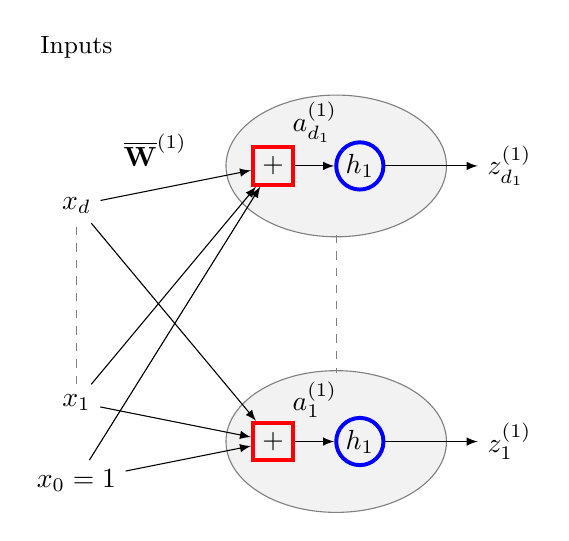
\begin{tikzpicture}[>=latex]

  % --- plain text labels (virtual nodes) ---
  \node (Label01) at (1,-1)  {$x_{0}=1$};
  \node (Label11) at (1, 0)  {$x_{1}$};
  \node (Labeld1) at (1, 2.5){$x_{d}$};
  \node (Label1)  at (1, 4.5){\small Inputs};

  % --- filled ellipses (light gray background) ---
  \fill[lightgray!20] (4.3,-.5) ellipse (1.4 and .9);
  \fill[lightgray!20] (4.3, 3)  ellipse (1.4 and .9);

  % --- ellipse outlines ---
  \draw[gray] (4.3,-.5) ellipse (1.4 and .9);
  \draw[gray] (4.3, 3)  ellipse (1.4 and .9);

  % --- summation boxes (red border, thick) ---
  \node[draw=red, line width=.5mm, inner sep=1.2mm] (Add12) at (3.5,-.5) {$+$};
  \node[draw=red, line width=.5mm, inner sep=1.2mm] (Addm2) at (3.5, 3)  {$+$};

  % --- activation circles (blue border) ---
  \node[draw=blue, line width=.5mm, circle, minimum size=6mm, inner sep=0pt] (Act12) at (4.6,-.5) {$h_{1}$};
  \node[draw=blue, line width=.5mm, circle, minimum size=6mm, inner sep=0pt] (Actm2) at (4.6, 3)  {$h_{1}$};

  % --- output labels ---
  \node (Label12) at (6.5,-.5) {$z_{1}^{(1)}$};
  \node (Label0m) at (6.5, 3)  {$z_{d_1}^{(1)}$};

  % --- invisible anchor nodes for the dashed vertical line ---
  \node (n1) at (4.3, 2.25) {};
  \node (n2) at (4.3, 0.25) {};

  % --- weight matrix label ---
  \node (beta1) at (2, 3.2) {$\mathbf{\overline{W}}^{(1)}$};

  % --- arrows from inputs to summation nodes ---
  \draw[->] (Label01) -- (Add12);
  \draw[->] (Label01) -- (Addm2);
  \draw[->] (Label11) -- (Add12);
  \draw[->] (Label11) -- (Addm2);
  \draw[->] (Labeld1) -- (Add12);
  \draw[->] (Labeld1) -- (Addm2);

  % --- arrows from summation to activation, with midpoint labels ---
  \draw[->] (Addm2) -- node[above=5pt] {$a_{d_1}^{(1)}$} (Actm2);
  \draw[->] (Add12) -- node[above=5pt] {$a_{1}^{(1)}$}   (Act12);

  % --- arrows from activation to output labels ---
  \draw[->] (Act12) -- (Label12);
  \draw[->] (Actm2) -- (Label0m);

  % --- dashed lines ---
  \draw[gray, dashed] (Label11) -- (Labeld1);
  \draw[gray, dashed] (n1)      -- (n2);

\end{tikzpicture}
\end{center}

\medskip
Once this mechanism is clear, the idea of depth becomes almost inevitable: we can \emph{iterate} the same construction, feeding the vector $\z^{(1)}$ into another layer of units, which computes new pre-activations and new nonlinear outputs. By stacking several such layers, we obtain a multilayer network. The depth of the resulting architecture is precisely the number of times this affine-then-nonlinear pattern is repeated.

The approach can be iterated, adding more layers with the same structure, and resulting in a multilayer network. Here, one additional hidden layer is added to the previous construction.
\begin{center}
\begin{tikzpicture}
     \Vertex[Math, x=5.1,y=0, color=xkcdLightGrey, opacity=.4, shape = rectangle, style={minimum width=6.5cm, minimum height=2.7cm, line width=.3pt,  draw=xkcdDarkGrey}]{A0}
\Vertex[Math, x=1,y=0, color=xkcdFadedBlue, opacity=.8, shape = rectangle, label = \x, fontsize=\footnotesize, style={minimum width=1.4cm, minimum height=3mm, line width=.1pt}]{B0}
 \Text[position=below,x=1,y=0, distance=1.2mm, fontsize=\scriptsize]{$d$}
 
 \Vertex[Math, x=2.75,y=0, color=xkcdTurquoise, opacity=.5, shape = rectangle, label = \W_1, fontsize=\footnotesize, style={minimum width=.9cm, minimum height=1.4cm, line width=1pt,  draw=xkcdReddish}]{B1}
 \Text[position=above,x=2.75,y=0, distance=7mm, fontsize=\scriptsize]{$d_1$}
 \Text[position=right,x=2.75,y=.5, distance=5mm, fontsize=\scriptsize]{$d$}
 
 \Edge[lw=.5pt, Direct](B0)(B1)
 
 \Vertex[Math, x=4,y=0, color=xkcdLightGrey, label = +, size = .4, opacity=.5, fontsize=\footnotesize, style={line width=.5pt}]{C}
 \Edge[lw=.5pt, Direct](B1)(C)
 
 \Vertex[Math, x=4,y=-1, color=xkcdTurquoise, label = b_1, opacity=.5, shape = rectangle, fontsize=\footnotesize, style={minimum width=9mm, minimum height=3mm, line width=1pt,  draw=xkcdReddish}]{B3}
 \Edge[lw=.5pt, Direct](B3)(C)
   
 \Vertex[Math, x=4.75,y=0, color=xkcdLightGrey, label = h_1, size = .4, opacity=.5, fontsize=\footnotesize, style={line width=.5pt}]{C1}
 \Edge[lw=.5pt, Direct](C)(C1)
 
 \Vertex[Math, x=6,y=0, color=xkcdTurquoise, opacity=.5, shape = rectangle, label = \W_2, fontsize=\footnotesize, style={minimum width=1.1cm, minimum height=.9cm, line width=1pt,  draw=xkcdReddish}]{B4}
 \Text[position=above,x=6,y=0, distance=5mm, fontsize=\scriptsize]{$d_2$}
 \Text[position=right,x=6,y=.4, distance=6mm, fontsize=\scriptsize]{$d_1$}
 \Edge[lw=.5pt, Direct](C1)(B4)
 
 \Vertex[Math, x=7.25,y=0, color=xkcdLightGrey, label = +, size = .4, opacity=.5, fontsize=\footnotesize, style={line width=.5pt}]{C2}
 \Edge[lw=.5pt, Direct](B4)(C2)
 
 \Vertex[Math, x=7.25,y=-1, color=xkcdTurquoise, label = b_2, opacity=.5, shape = rectangle, fontsize=\footnotesize, style={minimum width=9mm, minimum height=3mm, line width=1pt,  draw=xkcdReddish}]{B5}
 \Edge[lw=.5pt, Direct](B5)(C2)
   
 \Vertex[Math, x=8,y=0, color=xkcdLightGrey, label = h_2, size = .4, opacity=.5, fontsize=\footnotesize, style={line width=.5pt}]{C3}
 \Edge[lw=.5pt, Direct](C2)(C3)
 
 \Vertex[Math, x=9,y=0, color=xkcdTurquoise, opacity=.5, shape = rectangle, label = \w_3, fontsize=\footnotesize, style={minimum width=.4cm, minimum height=1.9cm, line width=1pt,  draw=xkcdReddish}]{B41}
 \Text[position=right,x=9,y=.7, distance=2mm, fontsize=\scriptsize]{$d_2$}
 \Edge[lw=.7pt, Direct](C3)(B41)
 
 \Vertex[Math, x=10,y=0, color=xkcdLightGrey, label = +, size = .4, opacity=.5, fontsize=\footnotesize, style={line width=.5pt}]{C21}
 \Edge[lw=.5pt, Direct](B41)(C21)
 
 \Vertex[Math, x=10,y=-1, color=xkcdTurquoise, label = b_3, opacity=.5, shape = rectangle, fontsize=\footnotesize, style={minimum width=3mm, minimum height=3mm, line width=1pt,  draw=xkcdReddish}]{B51}
 \Edge[lw=.5pt, Direct](B51)(C21)
   
 \Vertex[Math, x=10.75,y=0, color=xkcdLightGrey, label = \varphi, size = .4, opacity=.5, fontsize=\footnotesize, style={line width=.5pt}]{C31}
 \Edge[lw=.5pt, Direct](C21)(C31)
 
 \Vertex[Math, x=11.5,y=0, color=xkcdLipstickRed, opacity=.5, shape = rectangle, fontsize=\footnotesize, style={minimum width=3mm, minimum height=3mm, line width=.1pt}]{C6}
 \Edge[lw=.5pt, Direct](C31)(C6)  
\end{tikzpicture}
\end{center}

\medskip
At this point, the notation becomes slightly heavier, but the underlying operation is exactly the same as in the first layer, applied to a new input. The vector $\z^{(1)}$ now provides the input to the second layer, where $d_2$ \alert{hidden units} compute a new vector $\z^{(2)}=(z_1^{(2)}, \ldots, z_{d_2}^{(2)})^T$. The computation again splits into an affine step and a nonlinear step: first, the pre-activations are formed via
\begin{myequation}
a_{k}^{(2)}=\sum_{i=1}^{d_1}w_{ki}^{(2)}z_{i}^{(1)}+b_{k}^{(2)}={\ow_k^{(2)}}^T\overline{\z}^{(1)},
\end{myequation}
and then the nonlinearity is applied to each pre-activation:
\begin{myequation}
z_{k}^{(2)}=h_{2}({\ow_k^{(2)}}^T\overline{\z}^{(1)}).
\end{myequation}
Here $\overline{\z}^{(1)}$ denotes the augmented vector that includes the constant component used to incorporate the bias term into the weight vector, in perfect analogy with the first layer. Interpreting these formulas, each hidden unit in layer 2 is again a small GLM, but one that acts not on the raw input $\x$, but on the \emph{features} computed by the previous layer. This is precisely why depth is so often described in terms of ``learning representations'': each layer reshapes the information carried by its input into a new coordinate system that, ideally, makes the final prediction task progressively easier.

In most architectures, one chooses $h_2=h_1$, using the same activation function throughout all hidden layers. The output layer typically uses a different, task-dependent function $\varphi$. This convention is not mandatory, but it simplifies the architecture and is generally sufficient in practice, since the learned weight matrices already provide the flexibility needed to adapt the computation to the data.

The same structure extends naturally to any number of layers. If layer $r$ has $d_r$ units and receives the output vector $\z^{(r-1)}$ from the preceding layer, it computes pre-activations through
\begin{myequation}
a_{k}^{(r)}={\ow_k^{(r)}}^T\overline\z^{(r-1)},
\end{myequation}
and then applies the nonlinearity to produce outputs:
\begin{myequation}
z_{k}^{(r)}=h_{r}({\ow_k^{(r)}}^T\overline\z^{(r-1)}).
\end{myequation}
In words: affine map, then nonlinearity, repeated many times. This is the basic template of all multilayer networks, and the diagram below illustrates the general pattern for a generic inner layer $r$.

\begin{center}
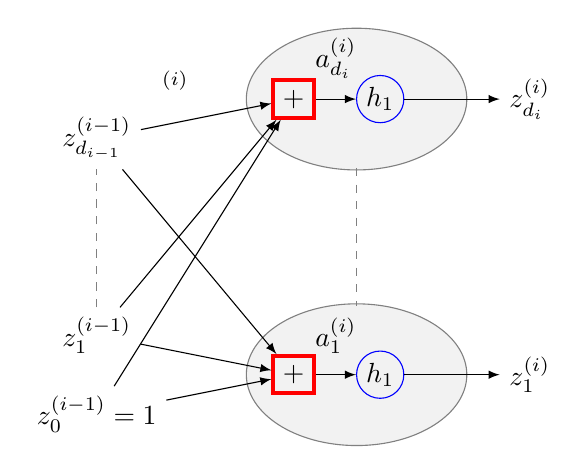
\begin{tikzpicture}[>=latex]

  % --- plain text labels (virtual nodes) ---
  \node (Label01) at (1,-1)  {$z_{0}^{(i-1)}=1$};
  \node (Label11) at (1, 0)  {$z_{1}^{(i-1)}$};
  \node (Labeld1) at (1, 2.5){$z_{d_{i-1}}^{(i-1)}$};

  % --- filled ellipses (light gray background) ---
  \fill[lightgray!20] (4.3,-.5) ellipse (1.4 and .9);
  \fill[lightgray!20] (4.3, 3)  ellipse (1.4 and .9);

  % --- ellipse outlines ---
  \draw[gray] (4.3,-.5) ellipse (1.4 and .9);
  \draw[gray] (4.3, 3)  ellipse (1.4 and .9);

  % --- summation boxes (red border, thick) ---
  \node[draw=red, line width=.5mm, inner sep=1.2mm] (Add12) at (3.5,-.5) {$+$};
  \node[draw=red, line width=.5mm, inner sep=1.2mm] (Addm2) at (3.5, 3)  {$+$};

  % --- activation circles (blue border) ---
  \node[draw=blue, circle, minimum size=6mm, inner sep=0pt] (Act12) at (4.6,-.5) {$h_{1}$};
  \node[draw=blue, circle, minimum size=6mm, inner sep=0pt] (Actm2) at (4.6, 3)  {$h_{1}$};

  % --- output labels ---
  \node (Label12) at (6.5,-.5) {$z_{1}^{(i)}$};
  \node (Label0m) at (6.5, 3)  {$z_{d_i}^{(i)}$};

  % --- invisible anchor nodes for the dashed vertical line ---
  \node (n1) at (4.3, 2.25) {};
  \node (n2) at (4.3, 0.25) {};

  % --- weight matrix label ---
  \node (beta1) at (2, 3.2) {$\overline{\W}^{(i)}$};

  % --- arrows from inputs to summation nodes ---
  \draw[->] (Label01) -- (Add12);
  \draw[->] (Label01) -- (Addm2);
  \draw[->] (Label11) -- (Add12);
  \draw[->] (Label11) -- (Addm2);
  \draw[->] (Labeld1) -- (Add12);
  \draw[->] (Labeld1) -- (Addm2);

  % --- arrows from summation to activation, with midpoint labels ---
  \draw[->] (Addm2) -- node[above=4pt] {$a_{d_i}^{(i)}$} (Actm2);
  \draw[->] (Add12) -- node[above=4pt] {$a_{1}^{(i)}$}   (Act12);

  % --- arrows from activation to output labels ---
  \draw[->] (Act12) -- (Label12);
  \draw[->] (Actm2) -- (Label0m);

  % --- dashed lines ---
  \draw[gray, dashed] (Label11) -- (Labeld1);
  \draw[gray, dashed] (n1)      -- (n2);

\end{tikzpicture}
\end{center}

\subsubsection*{Multilayer network structure: output layer}

After $D-1$ hidden layers have transformed the input through a sequence of learned representations, the final layer (layer $D$) produces the network output $\y=\z^{(D)}$. The computation in this last layer follows the same pattern as the hidden layers: affine combinations of the previous layer's outputs, followed by a nonlinearity. What changes is the choice of the final function $\varphi$, which must be tailored to the requirements of the task rather than to representational convenience. Formally,
\begin{myequation}
a_{k}^{(D)}={\ow_k^{(D)}}^T\overline\z^{(D-1)},
\end{myequation}
and then
\begin{myequation}
y_k=z_{k}^{(D)}=\varphi({\ow_k^{(D)}}^T\overline\z^{(D-1)}).
\end{myequation}
The vector $\z^{(D-1)}$ represents the last internal representation built by the network---the final, most abstract feature space---and the output layer reads it out in a way that is appropriate for the problem. The same expression can therefore represent very different models depending on $\varphi$, which is typically chosen as the identity function for regression (so that outputs can take any real value), a sigmoid for binary classification (so that the output can be interpreted as a probability in $(0,1)$), or a softmax for multiclass classification (so that outputs form a valid probability distribution over $K$ classes). While these choices may seem like a short list of options, they reflect a unified principle: $\varphi$ is chosen to enforce the geometric and probabilistic constraints that the output is required to satisfy.

\subsubsection*{Output layer: regression}

In regression, the output unit simply returns the affine pre-activation without any further transformation. In other words, the function $\varphi$ is the identity, and the output is
\begin{myequation}
y = a^{(D)} = {\ow^{(D)}}^T \overline\z^{(D-1)}.
\end{myequation}
One may interpret this as a linear regression model applied directly to the learned internal representation $\z^{(D-1)}$: the hidden layers have transformed the input into a feature space where the target quantity is (approximately) a linear function, and the output layer reads off this linear relationship. The following diagram illustrates the output layer for the regression case, where no nonlinearity node appears after the summation.

\begin{center}
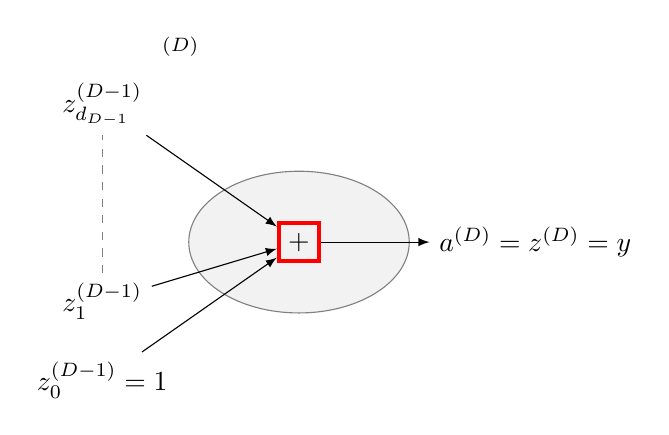
\begin{tikzpicture}[>=latex]

  % --- plain text labels (virtual nodes) ---
  \node (Label01) at (1,-1)  {$z_{0}^{(D-1)}=1$};
  \node (Label11) at (1, 0)  {$z_{1}^{(D-1)}$};
  \node (Labeld1) at (1, 2.5){$z_{d_{D-1}}^{(D-1)}$};

  % --- single filled ellipse (light gray background) ---
  \fill[lightgray!20] (3.5,.75) ellipse (1.4 and .9);

  % --- ellipse outline ---
  \draw[gray] (3.5,.75) ellipse (1.4 and .9);

  % --- summation box (red border, thick) ---
  \node[draw=red, line width=.5mm, inner sep=1.2mm] (Add12) at (3.5,.75) {$+$};

  % --- output label ---
  \node (Label12) at (6.5,.75) {$a^{(D)}=z^{(D)}=y$};

  % --- weight vector label ---
  \node (beta1) at (2, 3.2) {$\overline{\w}^{(D)}$};

  % --- arrows from inputs to summation node ---
  \draw[->] (Label01) -- (Add12);
  \draw[->] (Label11) -- (Add12);
  \draw[->] (Labeld1) -- (Add12);

  % --- arrow from summation to output ---
  \draw[->] (Add12) -- (Label12);

  % --- dashed line between input labels ---
  \draw[gray, dashed] (Label11) -- (Labeld1);

\end{tikzpicture}
\end{center}

\subsubsection*{Output layer: binary classification}

For binary classification, the affine score $a^{(D)}$ is converted into a number in $(0,1)$ by the sigmoid function $\sigma$. This is not merely a convenient squashing operation: it provides a probabilistic interpretation of the output, since the sigmoid maps any real number to a value strictly between zero and one, which can be read as the estimated probability that the input belongs to the positive class. This output convention ties naturally to the cross-entropy loss function, which is the standard training objective for binary classification and arises from the negative log-likelihood of a Bernoulli model.

\begin{center}
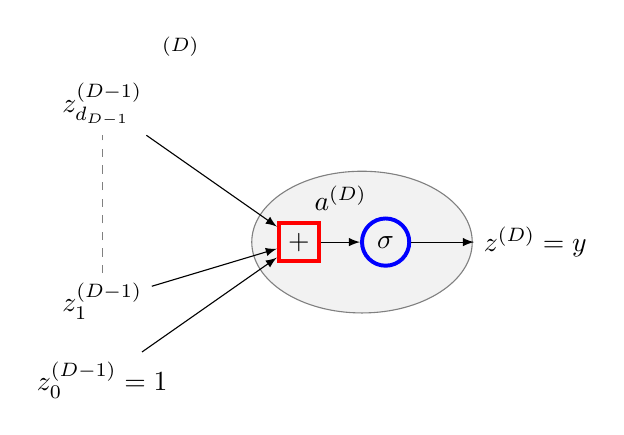
\begin{tikzpicture}[>=latex]

  % --- plain text labels (virtual nodes) ---
  \node (Label01) at (1,-1)  {$z_{0}^{(D-1)}=1$};
  \node (Label11) at (1, 0)  {$z_{1}^{(D-1)}$};
  \node (Labeld1) at (1, 2.5){$z_{d_{D-1}}^{(D-1)}$};

  % --- single filled ellipse (light gray background) ---
  \fill[lightgray!20] (4.3,.75) ellipse (1.4 and .9);

  % --- ellipse outline ---
  \draw[gray] (4.3,.75) ellipse (1.4 and .9);

  % --- summation box (red border, thick) ---
  \node[draw=red, line width=.5mm, inner sep=1.2mm] (Add12) at (3.5,.75) {$+$};

  % --- activation circle (blue border) ---
  \node[draw=blue, line width=.5mm, circle, minimum size=6mm, inner sep=0pt] (Act12) at (4.6,.75) {$\sigma$};

  % --- output label ---
  \node (Label12) at (6.5,.75) {$z^{(D)}=y$};

  % --- weight vector label ---
  \node (beta1) at (2, 3.2) {$\overline{\w}^{(D)}$};

  % --- arrows from inputs to summation node ---
  \draw[->] (Label01) -- (Add12);
  \draw[->] (Label11) -- (Add12);
  \draw[->] (Labeld1) -- (Add12);

  % --- arrow from summation to activation, with midpoint label ---
  \draw[->] (Add12) -- node[above=8pt] {$a^{(D)}$} (Act12);

  % --- arrow from activation to output ---
  \draw[->] (Act12) -- (Label12);

  % --- dashed line between input labels ---
  \draw[gray, dashed] (Label11) -- (Labeld1);

\end{tikzpicture}
\end{center}

\subsubsection*{Output layer: $K$-class classification}

For $K$-class classification, the output layer consists of $K$ units, each computing a scalar pre-activation $a_k^{(D)}$ that can be thought of as the network's raw ``score'' or ``logit'' for class $k$. These scores are then jointly transformed by the softmax function $s$, which normalizes them into a proper probability vector. Concretely,
\begin{myequation}
y_k = s_k(a_1^{(D)}, \ldots, a_K^{(D)}) = \frac{e^{a_k^{(D)}}}{\sum_{j=1}^{K} e^{a_j^{(D)}}}.
\end{myequation}
The normalization couples the outputs in a meaningful way: increasing one score raises the probability for that class at the expense of all others, which is exactly the competition structure one expects among mutually exclusive classes. This output convention again pairs naturally with the cross-entropy loss, now in its multiclass form, which arises from the negative log-likelihood of a categorical distribution.

\begin{center}
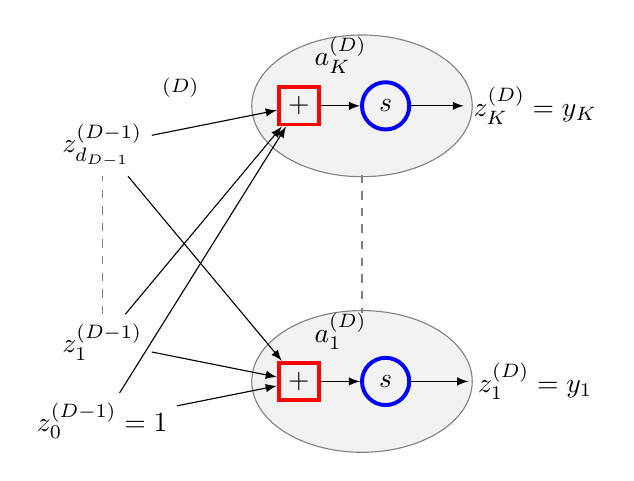
\begin{tikzpicture}[>=latex]

  % --- plain text labels (virtual nodes) ---
  \node (Label01) at (1,-1)  {$z_{0}^{(D-1)}=1$};
  \node (Label11) at (1, 0)  {$z_{1}^{(D-1)}$};
  \node (Labeld1) at (1, 2.5){$z_{d_{D-1}}^{(D-1)}$};

  % --- filled ellipses (light gray background) ---
  \fill[lightgray!20] (4.3,-.5) ellipse (1.4 and .9);
  \fill[lightgray!20] (4.3, 3)  ellipse (1.4 and .9);

  % --- ellipse outlines ---
  \draw[gray] (4.3,-.5) ellipse (1.4 and .9);
  \draw[gray] (4.3, 3)  ellipse (1.4 and .9);

  % --- summation boxes (red border, thick) ---
  \node[draw=red, line width=.5mm, inner sep=1.2mm] (Add12) at (3.5,-.5) {$+$};
  \node[draw=red, line width=.5mm, inner sep=1.2mm] (Addm2) at (3.5, 3)  {$+$};

  % --- softmax activation circles (blue border) ---
  \node[draw=blue, line width=.5mm, circle, minimum size=6mm, inner sep=0pt] (Act12) at (4.6,-.5) {$s$};
  \node[draw=blue, line width=.5mm, circle, minimum size=6mm, inner sep=0pt] (Actm2) at (4.6, 3)  {$s$};

  % --- output labels ---
  \node (Label12) at (6.5,-.5) {$z_{1}^{(D)}=y_1$};
  \node (Label0m) at (6.5, 3)  {$z_{K}^{(D)}=y_K$};

  % --- invisible anchor nodes for the dashed vertical line ---
  \node (n1) at (4.3, 2.25) {};
  \node (n2) at (4.3, 0.25) {};

  % --- weight matrix label ---
  \node (beta1) at (2, 3.2) {$\overline{\W}^{(D)}$};

  % --- arrows from inputs to summation nodes ---
  \draw[->] (Label01) -- (Add12);
  \draw[->] (Label01) -- (Addm2);
  \draw[->] (Label11) -- (Add12);
  \draw[->] (Label11) -- (Addm2);
  \draw[->] (Labeld1) -- (Add12);
  \draw[->] (Labeld1) -- (Addm2);

  % --- arrows from summation to activation, with midpoint labels ---
  \draw[->] (Addm2) -- node[above=8pt] {$a_{K}^{(D)}$} (Actm2);
  \draw[->] (Add12) -- node[above=8pt] {$a_{1}^{(D)}$}  (Act12);

  % --- arrows from activation to output labels ---
  \draw[->] (Act12) -- (Label12);
  \draw[->] (Actm2) -- (Label0m);

  % --- dashed lines ---
  \draw[gray, dashed] (Label11) -- (Labeld1);
  \draw[gray, dashed] (n1)      -- (n2);

\end{tikzpicture}
\end{center}

\subsection*{Three-layer networks}

A particularly important and widely studied architecture is the network consisting of three types of layers: an input layer, which simply provides $\x$; a single hidden layer, which computes a learned intermediate representation; and an output layer, which produces the final prediction $\y$. Despite the apparent modesty of having only one hidden layer, this architecture is already capable of representing highly expressive functions, because the hidden layer can learn data-dependent nonlinear features that are tailored to the task. This makes three-layer networks a natural first step beyond classical GLMs, and understanding their structure in detail provides essentially all the intuition needed to reason about deeper architectures.

To be concrete, consider $K$-class classification with a hidden layer of size $d_1$. Reading the network computation from input to output, the overall function computed for each class-$k$ output, $k=1,\ldots,K$, can be written in closed form as
\begin{myequation}
y_{k}=s\left(\sum_{j=1}^{d_1}w_{kj}^{(2)}h\left(\sum_{i=1}^{d}w_{ji}^{(1)}x_{i}+b_{j}^{(1)}\right)+b_{k}^{(2)}\right),
\end{myequation}
where $d_1$ is a structural hyperparameter specifying the number of hidden units, and $s$ denotes the softmax function. This expression repays careful reading from the inside out. The innermost sum, $\sum_{i=1}^{d}w_{ji}^{(1)}x_i+b_j^{(1)}$, is the pre-activation of hidden unit $j$, formed by taking an affine combination of all input coordinates. Applying $h$ to this quantity yields the $j$-th hidden unit's output, which constitutes one component of the learned representation. The outer sum $\sum_{j=1}^{d_1}w_{kj}^{(2)}h(\cdots)+b_k^{(2)}$ then linearly combines all $d_1$ hidden unit outputs to form the class-$k$ score. Finally, $s$ converts all $K$ class scores into a probability vector. In this way, the output of the network for each class arises from a two-step computation: feature extraction in the hidden layer, followed by linear classification in the feature space.

This structure can be given a unified interpretation: the three-layer network is a GLM in which the basis functions $h\bigl(\sum_i w_{ji}^{(1)} x_i + b_j^{(1)}\bigr)$ are not fixed in advance, as in classical models using polynomial or Fourier features, but are \emph{learned from data} through the parameters $\overline{\W}^{(1)}$. The hidden layer thus acts as an adaptive feature extractor, while the output layer performs softmax linear classification in the learned feature space. The key advantage over handcrafted feature maps is that the features discovered by the network are optimized jointly with the classifier, allowing the representation to be shaped by the task.

\begin{center}
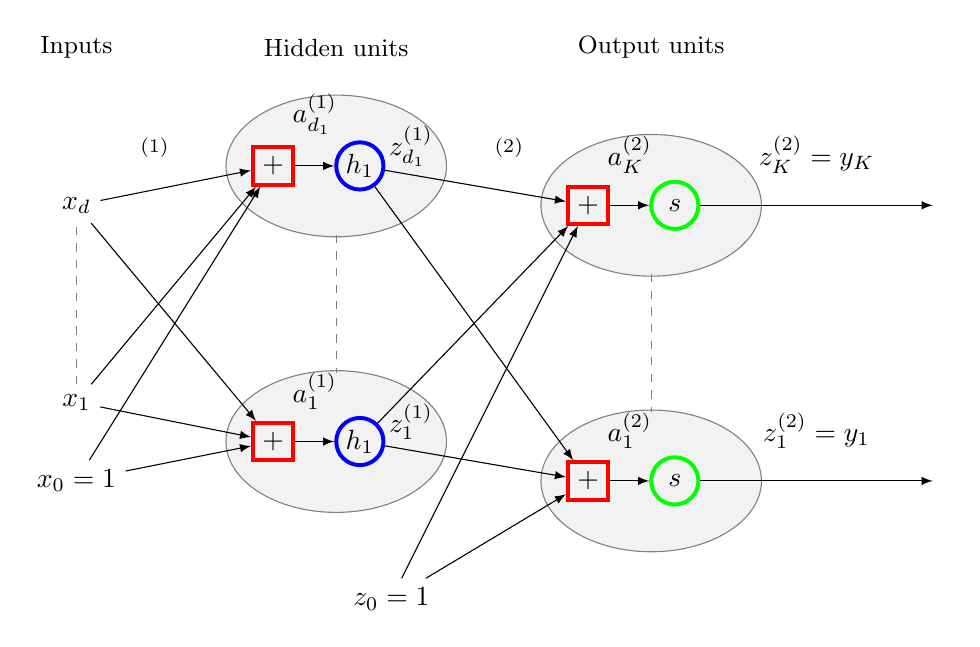
\begin{tikzpicture}[>=latex]

  % --- section header labels ---
  \node (Label1)  at (-2, 4.5) {\small Inputs};
  \node (Label2)  at (1.3, 4.5) {\small Hidden units};
  \node (Label3)  at (5.3, 4.5) {\small Output units};

  % --- input labels ---
  \node (Label01) at (-2,-1)  {$x_{0}=1$};
  \node (Label11) at (-2, 0)  {$x_{1}$};
  \node (Labeld1) at (-2, 2.5){$x_{d}$};

  % --- bias node for second layer ---
  \node (Label02) at (2,-2.5) {$z_{0}=1$};

  % --- filled ellipses (light gray background) ---
  \fill[lightgray!20] (1.3,-.5)  ellipse (1.4 and .9);
  \fill[lightgray!20] (1.3, 3)   ellipse (1.4 and .9);
  \fill[lightgray!20] (5.3, 2.5) ellipse (1.4 and .9);
  \fill[lightgray!20] (5.3,-1)   ellipse (1.4 and .9);

  % --- ellipse outlines ---
  \draw[gray] (1.3,-.5)  ellipse (1.4 and .9);
  \draw[gray] (1.3, 3)   ellipse (1.4 and .9);
  \draw[gray] (5.3, 2.5) ellipse (1.4 and .9);
  \draw[gray] (5.3,-1)   ellipse (1.4 and .9);

  % --- summation boxes, hidden layer (red border, thick) ---
  \node[draw=red, line width=.5mm, inner sep=1.2mm] (Add12) at (.5,-.5) {$+$};
  \node[draw=red, line width=.5mm, inner sep=1.2mm] (Addm2) at (.5, 3)  {$+$};

  % --- summation boxes, output layer (red border, thick) ---
  \node[draw=red, line width=.5mm, inner sep=1.2mm] (Addk3) at (4.5, 2.5) {$+$};
  \node[draw=red, line width=.5mm, inner sep=1.2mm] (Add13) at (4.5,-1)   {$+$};

  % --- activation circles, hidden layer (blue border) ---
  \node[draw=blue, line width=.5mm,  circle, minimum size=6mm, inner sep=0pt] (Act12) at (1.6,-.5) {$h_{1}$};
  \node[draw=blue, line width=.5mm,  circle, minimum size=6mm, inner sep=0pt] (Actm2) at (1.6, 3)  {$h_{1}$};

  % --- activation circles, output layer (green border) ---
  \node[draw=green, line width=.5mm, circle, minimum size=6mm, inner sep=0pt] (Actk3) at (5.6, 2.5) {$s$};
  \node[draw=green, line width=.5mm, circle, minimum size=6mm, inner sep=0pt] (Act13) at (5.6,-1)   {$s$};

  % --- hidden layer output labels ---
  \node (Label12) at (2.25,-.25)  {$z_{1}^{(1)}$};
  \node (Label0m) at (2.25, 3.25) {$z_{d_1}^{(1)}$};

  % --- output layer terminal labels (invisible anchors with labels on arrows) ---
  \node (Outputk) at (9, 2.5) {};
  \node (Output1) at (9,-1)   {};

  % --- invisible anchor nodes for dashed vertical lines ---
  \node (n1) at (1.3, 2.25) {};
  \node (n2) at (1.3, 0.25) {};
  \node (n3) at (5.3, 1.75) {};
  \node (n4) at (5.3,-.25)  {};

  % --- weight matrix labels ---
  \node (beta1) at (-1,  3.2) {$\overline{\W}^{(1)}$};
  \node (beta2) at (3.5, 3.2) {$\overline{\W}^{(2)}$};

  % --- arrows: inputs to hidden summation nodes ---
  \draw[->] (Label01) -- (Add12);
  \draw[->] (Label01) -- (Addm2);
  \draw[->] (Label11) -- (Add12);
  \draw[->] (Label11) -- (Addm2);
  \draw[->] (Labeld1) -- (Add12);
  \draw[->] (Labeld1) -- (Addm2);

  % --- arrows: hidden summation to hidden activation, with midpoint labels ---
  \draw[->] (Addm2) -- node[above=8pt] {$a_{d_1}^{(1)}$} (Actm2);
  \draw[->] (Add12) -- node[above=8pt] {$a_{1}^{(1)}$}   (Act12);

  % --- arrows: output summation to output activation, with midpoint labels ---
  \draw[->] (Addk3) -- node[above=8pt] {$a_{K}^{(2)}$} (Actk3);
  \draw[->] (Add13) -- node[above=8pt] {$a_{1}^{(2)}$}  (Act13);

  % --- arrows: output activation to terminal nodes, with output labels ---
  \draw[->] (Act13) -- node[above=8pt] {$z_{1}^{(2)}=y_{1}$} (Output1);
  \draw[->] (Actk3) -- node[above=8pt] {$z_{K}^{(2)}=y_{K}$} (Outputk);

  % --- arrows: hidden activations to output summation nodes ---
  \draw[->] (Act12) -- (Add13);
  \draw[->] (Act12) -- (Addk3);
  \draw[->] (Actm2) -- (Add13);
  \draw[->] (Actm2) -- (Addk3);

  % --- arrows: bias node to output summation nodes ---
  \draw[->] (Label02) -- (Add13);
  \draw[->] (Label02) -- (Addk3);

  % --- dashed lines ---
  \draw[gray, dashed] (Label11) -- (Labeld1);
  \draw[gray, dashed] (n1)      -- (n2);
  \draw[gray, dashed] (n3)      -- (n4);

\end{tikzpicture}
\end{center}



\subsubsection*{Approximating functions with neural networks}

Neural networks, despite the apparent simplicity of their basic building blocks, are sufficiently powerful models to act as \alert{universal approximators}. This expressive power does not reside in any single unit taken in isolation, but rather emerges from the collective effect of combining many simple nonlinear transformations through learnable linear combinations. The individual units are deliberately simple; it is the architecture as a whole that endows the network with its remarkable representational capacity.

The key theoretical result formalizing this idea is known as the \alert{universal approximation theorem}. In its most classical formulation, the theorem states that a feedforward neural network with a \emph{single} hidden layer, equipped with a non-polynomial nonlinear activation function such as the sigmoid or the hyperbolic tangent, can approximate any continuous function on a compact domain to arbitrary precision. This is a striking result, because it says that depth beyond one hidden layer is not, in principle, necessary for expressiveness: width alone suffices.

More precisely, let $f \colon \mathbb{R}^d \to \mathbb{R}$ be a continuous function defined on a compact set $K \subset \mathbb{R}^d$, and let $\varepsilon > 0$ be an arbitrary precision level. Then there exists an integer $d_1 > 0$ and a collection of parameters $\{w_{ji}^{(1)}, b_j^{(1)}, w_j^{(2)}, b^{(2)}\}$ such that the function implemented by a neural network of the form
\begin{myequation}
\hat f(\x)
=
\sum_{j=1}^{d_1} w_j^{(2)} \, h\!\left( \sum_{i=1}^{d} w_{ji}^{(1)} x_i + b_j^{(1)} \right)
+ b^{(2)}
\end{myequation}
satisfies
\begin{myequation}
\sup_{\x \in K} \lvert f(\x) - \hat f(\x) \rvert < \varepsilon.
\end{myequation}
Here $h$ denotes a sigmoidal activation function, such as the logistic sigmoid or the hyperbolic tangent, and the supremum is taken over all points $\x$ in the compact domain $K$.

The intuition underlying this result is most clearly seen by thinking of each hidden unit as a simple nonlinear feature detector. For sigmoidal activations, the function $h(\w^T \x + b)$ behaves like a smooth approximation of a step function, transitioning from one constant value to another across a hyperplane $\{\x : \w^T \x + b = 0\}$ in the input space. By appropriately choosing the weight vector $\w$ and the bias $b$, each unit can therefore be made sensitive to the presence of a particular linear feature in a specific part of the input domain, acting as a localizable bump or ridge function along a chosen direction.

By combining sufficiently many such units through the outer sum, the network constructs an increasingly rich set of basis functions that cover the input domain. Crucially, these basis functions are not fixed in advance but are instead learned from data: both the directions $\w_j^{(1)}$ and the thresholds $b_j^{(1)}$ are trained parameters. The output layer then forms a linear combination of these learned features. In this sense, a two-layer neural network can be viewed as a generalized linear model in which the basis functions are parameterized and adaptive rather than predefined. As the number of hidden units $d_1$ grows, the span of these basis functions becomes increasingly dense in the space of continuous functions on $K$, so that arbitrarily accurate approximation is possible for any target function $f$.

It is important to stress that the universal approximation theorem is an \emph{existence} result: it guarantees that a good set of parameters exists for any target function and any precision level, but it says nothing about how to find those parameters, nor does it provide any bound on the number of hidden units $d_1$ required to achieve a given approximation quality $\varepsilon$. In practice, the number of units needed may grow very rapidly with the complexity of the target function, the dimension $d$ of the input, and the required precision. Moreover, even if the right architecture is chosen, \emph{learning} the parameters from finite training data involves optimization challenges, regularization choices, and generalization considerations that go well beyond the scope of the theorem.

Finally, while the original formulations of the universal approximation theorem focused on sigmoidal activations and single-hidden-layer architectures, many extensions and variants of the result are now known. Analogous guarantees hold for other nonlinearities, including the rectified linear unit (ReLU), and for a variety of architectural configurations. Deeper architectures, interestingly, can often achieve comparable or even better approximation quality with far fewer total units than shallow networks, by exploiting the compositional and hierarchical structure of complex functions. Nevertheless, the universal approximation theorem remains a foundational result in the theory of neural networks, providing a rigorous justification for why even relatively shallow models can, in principle, represent extremely complex functional relationships.

\subsection*{Iterative methods to minimize $E(\overline{\W})$}

Once the architecture of a neural network has been fixed, learning reduces to determining the parameter values collected in $\overline{\W}$ (weights and biases) so as to minimize an error, or loss, function $E(\overline{\W})$. In principle this is an optimization problem like many others, but in practice neural networks present a particularly challenging landscape: $E(\overline{\W})$ is typically \emph{highly nonconvex}, it depends on the parameters through repeated compositions of nonlinear functions, and it often exhibits an intricate geometry with valleys, plateaus, and saddle regions. Understanding these difficulties is not merely an academic exercise: it directly informs the design of training procedures and the practical choices one makes when fitting a network to data.

A first source of difficulty is the presence of many \emph{local minima}. Because nonlinear hidden units create a complicated mapping from $\overline{\W}$ to the network outputs, the error surface may have many basins of attraction, and an algorithm that follows a local descent direction can converge to different solutions depending on the initialization. In this sense, the outcome of training is sensitive to where one starts in parameter space, and there is generally no guarantee that the solution found is globally optimal.

A second, subtler, source of complexity is that minima are often \emph{not unique} in a meaningful sense: for each local minimum there typically exist many \emph{equivalent} minima, corresponding to different parameter configurations that implement exactly the same input--output function. Two classical symmetries explain this phenomenon. First, since hidden units in the same layer are interchangeable, any permutation of the hidden units within a layer, together with the corresponding permutation of their incoming and outgoing weights, leaves the network function entirely unchanged: the same computation is performed, just with the units relabeled. Second, for many activation functions---in particular odd ones, and more generally whenever the sign change can be compensated by the next layer---flipping the signs of all incoming weights to a given hidden unit while simultaneously flipping the signs of all its outgoing weights leaves the overall computation invariant. These two symmetries together imply that the set of minimizers is not an isolated collection of points but rather a family of equivalent solutions, related by these discrete transformations. This contributes substantially to the irregularity and redundancy of the error surface, and it is one of the reasons why studying the geometry of neural network loss functions is a rich and active research area.

Because of these features, analytical minimization is generally out of reach. Unlike linear regression, where the normal equations yield a closed-form solution, neural network loss functions do not admit a tractable direct formula for their minimizers. One must therefore resort to iterative optimization methods. The core idea is to build a sequence of parameter vectors
\begin{myequation}
\overline{\W}^{(k+1)}=\overline{\W}^{(k)}+\Delta\overline{\W}^{(k)},
\end{myequation}
where the increment $\Delta\overline{\W}^{(k)}$ is designed so that $E(\overline{\W}^{(k+1)})<E(\overline{\W}^{(k)})$, at least approximately. Each step moves the parameters in a direction that reduces the loss, and the process is repeated until convergence or until some stopping criterion is met. Since the objective is nonconvex and algorithms can be sensitive to initialization, it is often good practice to run the same procedure from several different random starting points and compare the solutions obtained, in order to gain some confidence that a reasonable part of the parameter space has been explored.

\subsubsection*{Gradient descent}

Among iterative methods, gradient-based procedures play a central role because they exploit information about how $E(\overline{\W})$ changes locally when parameters are perturbed. The simplest and most widely used approach is \alert{gradient descent}. At each iteration, one conceptually performs two operations: first, one evaluates the derivatives of the error function with respect to all parameters at the current point $\overline{\W}^{(k)}$, computing the gradient $\nabla E(\overline{\W})\big|_{\overline{\W}^{(k)}}$; second, one updates the parameters by moving in the direction of steepest local decrease, that is, in the direction opposite to the gradient. The rationale is that the gradient points in the direction of greatest local increase of $E$, so its negative points toward the most immediate decrease.

In its basic form, the update rule reads
\begin{myequation}
\overline{\W}^{(k+1)}=\overline{\W}^{(k)}-\eta\nabla E(\overline{\W})\Big|_{\overline{\W}^{(k)}},
\end{myequation}
where $\eta>0$ is the \alert{learning rate}. The learning rate controls the size of the step taken in parameter space at each iteration, and its choice is critical: if $\eta$ is too small, learning proceeds in the right direction but at an excessively slow rate; if $\eta$ is too large, the method may overshoot minima, oscillate, or even diverge. Although this update rule is derived from a local linear (first-order) approximation of $E(\overline{\W})$, the nonconvex nature of the objective means that the global behavior of the algorithm cannot be guaranteed by such local reasoning alone. In practice, however, this simple idea is remarkably effective, and much of modern deep learning is built on variants and refinements of this basic scheme.

The main practical bottleneck in gradient descent is the computation of $\nabla E(\overline{\W})$. Since $E$ depends on a potentially very large number of parameters and is defined through multiple nested layers of computation, evaluating all partial derivatives naively would be computationally prohibitive. This requirement motivates the backpropagation algorithm discussed in the next section, which provides a systematic and efficient way to evaluate all partial derivatives simultaneously by carefully reusing intermediate computations from the forward pass.

\subsubsection*{On-line (stochastic) gradient descent}

A crucial observation is that the error function is often defined as a sum over the individual training examples. If the training set has $n$ elements, one typically writes
\begin{myequation}
E(\overline{\W})=\sum_{i=1}^{n}E_i(\overline{\W}),
\end{myequation}
where $E_i(\overline{\W})$ denotes the contribution to the total loss coming from the $i$-th observation, for instance a squared residual in regression or a cross-entropy term in classification. This additive structure immediately suggests a cheaper alternative to computing the full gradient at every step: instead of summing over all $n$ training examples before taking a step, one might take a step after processing only a single example, or a small group of examples.

In \alert{on-line} (or \alert{stochastic}) gradient descent, parameters are updated using only one training example at a time:
\begin{myequation}
\overline{\W}^{(k+1)}=\overline{\W}^{(k)}-\eta\nabla E_i(\overline{\W})\Big|_{\overline{\W}^{(k)}}.
\end{myequation}
This update can be interpreted as moving in the direction that most decreases the error for the specific data point currently being processed. Because each step is computed from a single term of the sum, it is much less expensive than a full gradient step, which requires summing over all $n$ terms. The price to pay is that the update direction $\nabla E_i$ is now a noisy, high-variance estimate of the true gradient $\nabla E$, so more iterations may be required before the parameters converge to a good solution.

Interestingly, this ``noise'' is not necessarily a drawback. In fact, the random fluctuations introduced by cycling through individual training examples can help the optimization process avoid getting trapped in poor local minima and can facilitate movement across flat regions or near saddle points---areas where the full gradient is small and a deterministic method would stall. For this reason, stochastic gradient descent is often effective and even preferable in large-scale learning, where computing the exact gradient over the entire dataset at each iteration would be computationally prohibitive regardless of the resulting step quality.

\subsubsection*{Batch gradient descent}

Between the two extremes of using the whole dataset and using a single observation, one can compute gradients on a subset---a \alert{mini-batch}---$B$ of the training set. The corresponding update is
\begin{myequation}
\overline{\W}^{(k+1)}=\overline{\W}^{(k)}-\eta\sum_{\x_i\in B}\nabla E_i(\overline{\W})\Big|_{\overline{\W}^{(k)}}.
\end{myequation}
In this form, the method trades off computational cost against the variance of the gradient estimate: larger batches provide a more accurate estimate of the full gradient and lead to more stable updates, while smaller batches provide cheaper and more frequent updates with higher noise. In many practical settings, using mini-batches strikes a favorable balance, yielding both efficient implementations---since modern hardware is optimized for batch matrix operations---and stable learning dynamics. The batch size is thus an important hyperparameter that must be tuned alongside the learning rate and the network architecture.

\subsection*{Computing gradients}

To apply any gradient-based optimization method, one must compute the partial derivatives of the error with respect to all parameters of the network. In particular, for each layer $r$ and for all relevant indices $i$ and $j$, we need the quantities
\begin{myequation}
\frac{\partial E(\overline{\W})}{\partial w_{ij}^{(r)}}
\end{myequation}
and
\begin{myequation}
\frac{\partial E(\overline{\W})}{\partial b_{j}^{(r)}}.
\end{myequation}
These derivatives must be evaluated repeatedly during learning, at varying parameter configurations $\overline{\W}^{(k)}$, which makes it essential to have formulas that can be computed efficiently and reliably.

For the sake of clarity, we begin the derivation at the output layer and work our way backward. As we shall see, the derivatives with respect to the weights can be expressed naturally in terms of derivatives with respect to the \emph{pre-activation values} at each layer. In particular, a convenient and natural starting point is the derivative of the loss with respect to the final-layer pre-activations,
\begin{myequation}
\frac{\partial E(\overline{\W})}{\partial a_i^{(D)}},
\end{myequation}
that is, the sensitivity of the cost function to each value $a_1^{(D)},\ldots,a_{d_D}^{(D)}$ entering the output nonlinearity. Once these quantities are known, they can be propagated backward through the network to compute the corresponding derivatives for all earlier layers. We now work out these output-layer derivatives for the three main cases.

\subsubsection*{Regression}

\begin{center}
\begin{tikzpicture}[x=1.5cm,y=.7cm]
    \node[fill=xkcdBuff,circle, draw,minimum size=18,inner sep=0.1,outer sep=0.6, thick, opacity=0.4, text opacity=1] (N00-1) at (0,0) {\small$a^{(D)}$};
    \node[fill=xkcdCobalt,circle, draw,minimum size=18,inner sep=0.1,outer sep=0.6, thick, opacity=0.4, text opacity=1] (N0-1) at (1,0) {\small$z^{(D)}$};
    \node[fill=xkcdLipstick,circle, draw,minimum size=18,inner sep=0.5,outer sep=0.6, thick, opacity=0.4, text opacity=1] (N1-3) at (2.5,0) {\small$E$};
    \node[fill=xkcdOrange,circle, draw,minimum size=18,inner sep=0.5,outer sep=0.6, thick, opacity=0.4, text opacity=1] (N2-1) at (3.5,1.5) {\small$t$};
    \draw[->, connect, line width=0.05] (N00-1) -- (N0-1);
    \draw[->, connect, line width=0.05] (N0-1) -- (N1-3);
    \draw[->, connect, line width=0.05] (N2-1) -- (N1-3);
\end{tikzpicture}
\end{center}

\bigskip
In regression, the output activation is passed through the identity function, so the network prediction is simply $y=z^{(D)}=a^{(D)}$. There is no nonlinearity at the output, and the pre-activation is directly interpreted as the predicted value. If we adopt the squared error loss for a single training example with target $t$,
\begin{myequation}
E=\frac{1}{2}(y-t)^2=\frac{1}{2}(z^{(D)}-t)^2=\frac{1}{2}(a^{(D)}-t)^2,
\end{myequation}
then differentiation with respect to the output pre-activation is immediate and yields
\begin{myequation}
{\color{xkcdTeal}\frac{\partial E}{\partial a^{(D)}}}=a^{(D)}-t=z^{(D)}-t.
\end{myequation}
This expression has a clean intuitive meaning: the derivative of the squared loss is simply the signed prediction error, that is, the amount by which the network output overshoots or undershoots the target. The factor of $\frac{1}{2}$ in the loss was chosen precisely to cancel the factor of $2$ that arises from differentiation, keeping the formula tidy.

\subsubsection*{Binary classification}

\begin{center}
\begin{tikzpicture}[x=1.5cm,y=.7cm]
    \node[fill=xkcdBuff,circle, draw,minimum size=18,inner sep=0.1,outer sep=0.6, thick, opacity=0.4, text opacity=1] (N00-1) at (0,0) {\small$a^{(D)}$};
    \node[fill=xkcdCobalt,circle, draw,minimum size=18,inner sep=0.1,outer sep=0.6, thick, opacity=0.4, text opacity=1] (N0-1) at (1,0) {\small$z^{(D)}$};
    \node[fill=xkcdLipstick,circle, draw,minimum size=18,inner sep=0.5,outer sep=0.6, thick, opacity=0.4, text opacity=1] (N1-3) at (2.5,0) {\small$E$};
    \node[fill=xkcdOrange,circle, draw,minimum size=18,inner sep=0.5,outer sep=0.6, thick, opacity=0.4, text opacity=1] (N2-1) at (3.5,1.5) {\small$t$};
    \draw[->, connect, line width=0.05] (N00-1) -- (N0-1);
    \draw[->, connect, line width=0.05] (N0-1) -- (N1-3);
    \draw[->, connect, line width=0.05] (N2-1) -- (N1-3);
\end{tikzpicture}
\end{center}

\bigskip
In binary classification, the output pre-activation is passed through the logistic sigmoid, so that $y=z^{(D)}=\sigma(a^{(D)})$ lies in $(0,1)$ and can be interpreted as the network's estimated probability that the input belongs to the positive class. The natural loss function in this setting is the binary cross-entropy,
\begin{align*}
E&=-(t\log y+(1-t)\log (1-y))=-(t\log z^{(D)}+(1-t)\log (1-z^{(D)})).
\end{align*}
Differentiating with respect to the output $z^{(D)}$ gives
\begin{align*}
\frac{\partial E}{\partial z^{(D)}}&=-\left(\frac{t}{z^{(D)}}-\frac{1-t}{1-z^{(D)}}\right)=\frac{z^{(D)}-t}{z^{(D)}(1-z^{(D)})}.
\end{align*}
This expression involves the factor $z^{(D)}(1-z^{(D)})$ in the denominator, which is precisely the variance of a Bernoulli random variable with success probability $z^{(D)}$. To obtain the derivative with respect to the pre-activation $a^{(D)}$, we use the chain rule together with the well-known identity for the sigmoid derivative,
\begin{myequation}
\frac{\partial z^{(D)}}{\partial a^{(D)}}=\sigma(a^{(D)})(1-\sigma(a^{(D)}))=z^{(D)}(1-z^{(D)}),
\end{myequation}
which yields
\begin{myequation}
{\color{xkcdTeal}\frac{\partial E}{\partial a^{(D)}}}
=
\frac{\partial E}{\partial z^{(D)}}\frac{\partial z^{(D)}}{\partial a^{(D)}}
=\frac{z^{(D)}-t}{z^{(D)}(1-z^{(D)})}\cdot z^{(D)}(1-z^{(D)})
=z^{(D)}-t.
\end{myequation}
The $z^{(D)}(1-z^{(D)})$ factors cancel perfectly, and again the derivative reduces to a simple difference between the network output and the target. This elegant cancellation is not a coincidence: it is a direct consequence of choosing the cross-entropy loss as the natural companion to the sigmoid output, a pairing that arises from the maximum-likelihood interpretation of the model. It is one of the principal reasons why the sigmoid--cross-entropy combination is so widely used in practice.

\subsubsection*{$K$-class classification}

\begin{center}
\begin{tikzpicture}[x=1.5cm,y=1.2cm]
    \node[fill=xkcdBuff,circle, draw,minimum size=18,inner sep=0.1,outer sep=0.6, thick, opacity=0.4, text opacity=1] (N00-1) at (0,0) {\small$a_{0}^{(D)}$};
    \node[fill=xkcdBuff,circle, draw,minimum size=18,inner sep=0.5,outer sep=0.6, thick, opacity=0.4, text opacity=1] (N00-2) at (0,-1) {\small$a_{1}^{(D)}$};
    \node[fill=xkcdBuff,circle, draw,minimum size=18,inner sep=0.5,outer sep=0.6, thick, opacity=0.4, text opacity=1] (N00-3) at (0,-2.5) {\small$a_{i}^{(D)}$};
    \node[fill=xkcdBuff,circle, draw,minimum size=18,inner sep=0.5,outer sep=0.6, thick, opacity=0.4, text opacity=1] (N00-4) at (0,-4) {\small$a_{K}^{(D)}$};
    \path (N00-2) --++ (N00-3) node[midway,scale=1] {$\vdots$};
    \path (N00-3) --++ (N00-4) node[midway,scale=1] {$\vdots$};
    \node[fill=xkcdCobalt,circle, draw,minimum size=18,inner sep=0.1,outer sep=0.6, thick, opacity=0.4, text opacity=1] (N0-1) at (1,0) {\small$z_{0}^{(D)}$};
    \node[fill=xkcdCobalt,circle, draw,minimum size=18,inner sep=0.5,outer sep=0.6, thick, opacity=0.4, text opacity=1] (N0-2) at (1,-1) {\small$z_{1}^{(D)}$};
    \node[fill=xkcdCobalt,circle, draw,minimum size=18,inner sep=0.5,outer sep=0.6, thick, opacity=0.4, text opacity=1] (N0-3) at (1,-2.5) {\small$z_{i}^{(D)}$};
    \node[fill=xkcdCobalt,circle, draw,minimum size=18,inner sep=0.5,outer sep=0.6, thick, opacity=0.4, text opacity=1] (N0-4) at (1,-4) {\small$z_{K}^{(D)}$};
    \path (N0-2) --++ (N0-3) node[midway,scale=1] {$\vdots$};
    \path (N0-3) --++ (N0-4) node[midway,scale=1] {$\vdots$};
    \node[fill=xkcdLipstick,circle, draw,minimum size=18,inner sep=0.5,outer sep=0.6, thick, opacity=0.4, text opacity=1] (N1-3) at (2.5,-1) {\small$E$};
    \node[fill=xkcdOrange,circle, draw,minimum size=18,inner sep=0.5,outer sep=0.6, thick, opacity=0.4, text opacity=1] (N2-1) at (3.5,.5) {\small$t_{0}$};
    \node[fill=xkcdOrange,circle, draw,minimum size=18,inner sep=0.5,outer sep=0.6, thick, opacity=0.4, text opacity=1] (N2-2) at (3.5,-.5) {\small$t_{1}$};
    \node[fill=xkcdOrange,circle, draw,minimum size=18,inner sep=0.5,outer sep=0.6, thick, opacity=0.4, text opacity=1] (N2-3) at (3.5,-2) {\small$t_{i}$};
    \node[fill=xkcdOrange,circle, draw,minimum size=18,inner sep=0.5,outer sep=0.6, thick, opacity=0.4, text opacity=1] (N2-4) at (3.5,-3.5) {\small$t_{K}$};
    \path (N2-2) --++ (N2-3) node[midway,scale=1] {$\vdots$};
    \path (N2-3) --++ (N2-4) node[midway,scale=1] {$\vdots$};
    \foreach \j in {1,...,4}{
        \foreach \i in {1,...,4}{
            \draw[->, connect, line width=0.05] (N00-\i) -- (N0-\j);
        }
        \draw[->, connect, line width=0.05] (N0-\j) -- (N1-3);
        \draw[->, connect, line width=0.05] (N2-\j) -- (N1-3);
    }
\end{tikzpicture}
\end{center}

In $K$-class classification, the output layer uses the softmax transformation to convert the $K$ pre-activations into a probability distribution over classes. The softmax is defined component-wise as
\begin{myequation}
y_i=z_i^{(D)}=\frac{e^{a_i^{(D)}}}{\sum_{j=1}^Ke^{a_j^{(D)}}},
\end{myequation}
so that all outputs are strictly positive and sum to one. With one-hot (or, more generally, probability) targets $\t=(t_1,\ldots,t_K)$, the multiclass cross-entropy loss is
\begin{myequation*}
E=-\sum_{i=1}^Kt_i\log z_i^{(D)}.
\end{myequation*}
Differentiating with respect to the softmax outputs gives
\begin{myequation*}
\frac{\partial E}{\partial z_i^{(D)}}=-\frac{t_i}{z_i^{(D)}}.
\end{myequation*}
To propagate the derivatives through the softmax layer, we need the Jacobian of the softmax outputs with respect to the pre-activations. A direct computation, distinguishing between the diagonal and off-diagonal cases, gives
\begin{myalign}
\frac{\partial z_i^{(D)}}{\partial a_i^{(D)}}&=\frac{e^{a_i^{(D)}}\sum_{j=1}^Ke^{a_j^{(D)}}-e^{a_i^{(D)}}e^{a_i^{(D)}}}{\left(\sum_{j=1}^Ke^{a_j^{(D)}}\right)^2}
=z_i^{(D)}(1-z_i^{(D)}),\\
\frac{\partial z_i^{(D)}}{\partial a_j^{(D)}}&=\frac{-e^{a_i^{(D)}}e^{a_j^{(D)}}}{\left(\sum_{j=1}^Ke^{a_j^{(D)}}\right)^2}
=-z_i^{(D)}z_j^{(D)},
\hspace{2cm}
i\not=j.
\end{myalign}
The first formula shows that the softmax output $z_i^{(D)}$ increases with its own pre-activation in a manner analogous to the sigmoid, while the second formula reflects the competitive nature of the softmax: increasing the pre-activation $a_j^{(D)}$ of class $j$ suppresses the output probability of all other classes $i \neq j$. Applying the chain rule, and carefully summing over all output units since each pre-activation $a_i^{(D)}$ affects all softmax outputs, yields
\begin{myalign}
{\color{xkcdTeal}\frac{\partial E}{\partial a_i^{(D)}}}
&=-\sum_{j=1}^K\frac{\partial E}{\partial z_j^{(D)}}\frac{\partial z_j^{(D)}}{\partial a_i^{(D)}}
=-\sum_{j=1}^K\frac{t_j}{z_j^{(D)}}\frac{\partial z_j^{(D)}}{\partial a_i^{(D)}}\\
&=-\frac{t_i}{z_i^{(D)}}z_i^{(D)}(1-z_i^{(D)})+\sum_{\substack{1\leq j\leq K\\j\not=i}}\frac{t_j}{z_j^{(D)}}z_i^{(D)}z_j^{(D)}\\
&=-t_i(1-z_i^{(D)})+\sum_{\substack{1\leq j\leq K\\j\not=i}}t_jz_i^{(D)}
=z_i^{(D)}\sum_{j=1}^Kt_j-t_i
=z_i^{(D)}-t_i,
\end{myalign}
where in the last step we used the fact that the target vector satisfies $\sum_{j=1}^K t_j = 1$ (since it represents a probability distribution or a one-hot encoding). Once more, the result has the clean form ``prediction minus target'', applied component-wise across all $K$ classes. The structural similarity across all three cases---regression, binary classification, and multiclass classification---is not a coincidence: it reflects the fact that in each case the loss is chosen to be the negative log-likelihood of the appropriate exponential family model, and the resulting derivative always takes the form of a residual.

\subsection*{Backpropagation}

Having identified the derivatives of the loss with respect to the final-layer pre-activations, the remaining task is to propagate these derivatives backward, layer by layer, until one obtains derivatives with respect to every weight and bias in the network. This procedure is known as \alert{backpropagation}, and it is the algorithmic engine that makes gradient-based training of deep networks computationally feasible.

Backpropagation can be interpreted as a backward flow of information through the computational graph defined by the network. In the \emph{forward pass}, inputs are fed through the network from the first layer to the last, computing and storing the pre-activations $a_j^{(r)}$ and the outputs $z_j^{(r)}$ at every layer $r$. These stored intermediate values are essential, because they are reused in the backward pass. In the \emph{backward pass}, one propagates \emph{error signals}---derivatives of $E$ with respect to intermediate pre-activations---from the output layer back toward the input layer, one layer at a time.

Beyond its primary role in training, the same mechanism can be used more broadly. For instance, one can apply backpropagation to compute derivatives of the network outputs with respect to input variables (producing Jacobians), or with additional bookkeeping to compute second-order derivatives (Hessians) at a given parameter configuration. What makes backpropagation especially valuable from a practical standpoint is its computational efficiency: it computes all partial derivatives simultaneously, with a total cost proportional to the number of parameters, rather than proportional to the square of the number of parameters as a naive finite-difference scheme would require.

We now show in detail how the backward recursion works. The key claim is that, for any layer $r$, knowing the current weight matrices and the values $a_i^{(r)}, z_i^{(r)}$ produced during the forward pass, the knowledge of the derivatives
\begin{myequation}
{\color{xkcdTeal}\frac{\partial E}{\partial a_j^{(r)}}}\hspace{2cm}1\leq j\leq d_r
\end{myequation}
is sufficient to compute both the derivatives of $E$ with respect to all weights and biases at layer $r$,
\begin{myequation}
{\color{xkcdLipstick}\frac{\partial E}{\partial w_{ij}^{(r)}}}\hspace{2cm}0\leq i\leq d_{r-1},\ 1\leq j\leq d_r,
\end{myequation}
and the derivatives needed to continue the backward pass one layer earlier,
\begin{myequation}
{\color{xkcdTeal}\frac{\partial E}{\partial a_i^{(r-1)}}}\hspace{2cm}1\leq i\leq d_{r-1},
\end{myequation}
where $d_s$ denotes the number of units at the $s$-th layer. Once the backward recursion is initialized at the output layer using the formulas derived in the previous section, it can be applied layer by layer all the way back to the first layer.

\subsubsection*{Backpropagation at layer $r$}

\begin{center}
\begin{tikzpicture}[x=2.2cm,y=1.2cm]
    \node[fill=xkcdOrange,circle, draw,minimum size=25,inner sep=0.1,outer sep=0.6, thick, opacity=0.4, text opacity=1] (N00-1) at (0,0) {\small$a_{0}^{(r-1)}$};
    \node[fill=xkcdOrange,circle, draw,minimum size=25,inner sep=0.5,outer sep=0.6, thick, opacity=0.4, text opacity=1] (N00-2) at (0,-1) {\small$a_{1}^{(r-1)}$};
    \node[fill=xkcdOrange,circle, draw,minimum size=25,inner sep=0.5,outer sep=0.6, thick, opacity=0.4, text opacity=1] (N00-3) at (0,-2.5) {\small$a_{i}^{(r-1)}$};
    \node[fill=xkcdOrange,circle, draw,minimum size=25,inner sep=0.5,outer sep=0.6, thick, opacity=0.4, text opacity=1] (N00-4) at (0,-4) {\small$a_{d_{r-1}}^{(r-1)}$};
    \path (N00-2) --++ (N00-3) node[midway,scale=1.2] {$\vdots$};
    \path (N00-3) --++ (N00-4) node[midway,scale=1.2] {$\vdots$};
    \node[fill=xkcdTeal,circle, draw,minimum size=15,inner sep=0.1,outer sep=0.6, thick, opacity=0.2, text opacity=1] (N0-0) at (1,1) {\small$1$};
    \node[fill=xkcdTeal,circle, draw,minimum size=25,inner sep=0.1,outer sep=0.6, thick, opacity=0.4, text opacity=1] (N0-1) at (1,0) {\small$z_{0}^{(r-1)}$};
    \node[fill=xkcdTeal,circle, draw,minimum size=25,inner sep=0.5,outer sep=0.6, thick, opacity=0.4, text opacity=1] (N0-2) at (1,-1) {\small$z_{1}^{(r-1)}$};
    \node[fill=xkcdTeal,circle, draw,minimum size=25,inner sep=0.5,outer sep=0.6, thick, opacity=0.4, text opacity=1] (N0-3) at (1,-2.5) {\small$z_{i}^{(r-1)}$};
    \node[fill=xkcdTeal,circle, draw,minimum size=25,inner sep=0.5,outer sep=0.6, thick, opacity=0.4, text opacity=1] (N0-4) at (1,-4) {\small$z_{d_{r-1}}^{(r-1)}$};
    \path (N0-2) --++ (N0-3) node[midway,scale=1.2] {$\vdots$};
    \path (N0-3) --++ (N0-4) node[midway,scale=1.2] {$\vdots$};
    \node[fill=xkcdBuff,circle, draw,minimum size=25,inner sep=0.5,outer sep=0.6, thick, opacity=0.4, text opacity=1] (N1-1) at (2.5,0) {\small$a_{0}^{(r)}$};
    \node[fill=xkcdBuff,circle, draw,minimum size=25,inner sep=0.5,outer sep=0.6, thick, opacity=0.4, text opacity=1] (N1-2) at (2.5,-1) {\small$a_{1}^{(r)}$};
    \node[fill=xkcdBuff,circle, draw,minimum size=25,inner sep=0.5,outer sep=0.6, thick, opacity=0.4, text opacity=1] (N1-3) at (2.5,-2.5) {\small$a_{j}^{(r)}$};
    \node[fill=xkcdBuff,circle, draw,minimum size=25,inner sep=0.5,outer sep=0.6, thick, opacity=0.4, text opacity=1] (N1-4) at (2.5,-4) {\small$a_{d_r}^{(r)}$};
    \path (N1-2) --++ (N1-3) node[midway,scale=1.2] {$\vdots$};
    \path (N1-3) --++ (N1-4) node[midway,scale=1.2] {$\vdots$};
    \node[fill=xkcdCobalt,circle, draw,minimum size=25,inner sep=0.5,outer sep=0.6, thick, opacity=0.4, text opacity=1] (N2-1) at (3.5,0) {\small$z_{0}^{(r)}$};
    \node[fill=xkcdCobalt,circle, draw,minimum size=25,inner sep=0.5,outer sep=0.6, thick, opacity=0.4, text opacity=1] (N2-2) at (3.5,-1) {\small$z_{1}^{(r)}$};
    \node[fill=xkcdCobalt,circle, draw,minimum size=25,inner sep=0.5,outer sep=0.6, thick, opacity=0.4, text opacity=1] (N2-3) at (3.5,-2.5) {\small$z_{j}^{(r)}$};
    \node[fill=xkcdCobalt,circle, draw,minimum size=25,inner sep=0.5,outer sep=0.6, thick, opacity=0.4, text opacity=1] (N2-4) at (3.5,-4) {\small$z_{d_r}^{(r)}$};
    \path (N2-2) --++ (N2-3) node[midway,scale=1.2] {$\vdots$};
    \path (N2-3) --++ (N2-4) node[midway,scale=1.2] {$\vdots$};
    \foreach \j in {1,...,4}{
        \foreach \i in {0,...,4}{
            \draw[->, connect, line width=0.05] (N0-\i) -- (N1-\j);
        }
        \draw[->, connect, line width=0.05] (N1-\j) -- (N2-\j);
        \draw[->, connect, line width=0.05] (N00-\j) -- (N0-\j);
    }
\end{tikzpicture}
\end{center}

At layer $r$, each pre-activation $a_j^{(r)}$ is computed as an affine combination of the outputs from the previous layer. Recalling the notation introduced earlier,
\begin{myequation*}
a_j^{(r)}=\sum_{i=1}^{d_{r-1}}w_{ij}^{(r)}z_i^{(r-1)}+b_j^{(r)}.
\end{myequation*}
Differentiating this expression with respect to each parameter gives
\begin{myequation*}
\frac{\partial a_j^{(r)}}{\partial w_{ij}^{(r)}}=z_i^{(r-1)},
\hspace{1cm}
\frac{\partial a_j^{(r)}}{\partial b_j^{(r)}}=1.
\end{myequation*}
The first identity states that the effect of a small change in the weight $w_{ij}^{(r)}$ on the pre-activation $a_j^{(r)}$ is proportional to the output $z_i^{(r-1)}$ feeding into that weight: a large input amplifies the sensitivity to the corresponding weight. The second identity simply reflects the additive and direct role of the bias term.

By the chain rule, if the derivatives ${\color{xkcdTeal}\frac{\partial E}{\partial a_j^{(r)}}}$ are known, the derivatives with respect to all weights and biases at layer $r$ are obtained immediately as
\begin{myalign}
{\color{xkcdLipstick}\frac{\partial E}{\partial w_{ij}^{(r)}}}
&=
{\color{xkcdTeal}\frac{\partial E}{\partial a_j^{(r)}}}
\frac{\partial a_j^{(r)}}{\partial w_{ij}^{(r)}}
=
{\color{xkcdTeal}\frac{\partial E}{\partial a_j^{(r)}}}z_i^{(r-1)},\\
{\color{xkcdLipstick}\frac{\partial E}{\partial b_j^{(r)}}}
&=
{\color{xkcdTeal}\frac{\partial E}{\partial a_j^{(r)}}}
\frac{\partial a_j^{(r)}}{\partial b_j^{(r)}}
=
{\color{xkcdTeal}\frac{\partial E}{\partial a_j^{(r)}}}.
\end{myalign}
These formulas express one of the fundamental patterns of backpropagation: the gradient on a weight connecting unit $i$ (in layer $r-1$) to unit $j$ (in layer $r$) equals the error signal at the destination unit $j$ multiplied by the value arriving through that connection from unit $i$. In other words, a weight is updated in proportion to both how much ``blame'' the destination unit carries and how strongly the source unit was active. This is reminiscent of classical Hebbian ideas, here given a precise gradient-based justification.

To continue the backward propagation to the preceding layer, one needs to determine how $E$ changes with respect to the outputs $z_i^{(r-1)}$ of layer $r-1$. Since $a_j^{(r)}$ depends on $z_i^{(r-1)}$ through the weight $w_{ij}^{(r)}$, we have $\frac{\partial a_j^{(r)}}{\partial z_i^{(r-1)}}=w_{ij}^{(r)}$, and summing over all units $j$ in layer $r$ (since $z_i^{(r-1)}$ influences every pre-activation in the next layer),
\begin{myequation}
\frac{\partial E}{\partial z_i^{(r-1)}}
=
\sum_{j=1}^{d_r}
{\color{xkcdTeal}\frac{\partial E}{\partial a_j^{(r)}}}
\frac{\partial a_j^{(r)}}{\partial z_i^{(r-1)}}
=
\sum_{j=1}^{d_r}{\color{xkcdTeal}\frac{\partial E}{\partial a_j^{(r)}}}w_{ij}^{(r)}.
\end{myequation}
This step propagates the error signal from layer $r$ back to the outputs of layer $r-1$: unit $i$'s share of the error is a weighted sum of all the error signals at layer $r$, with the weights given by the connections $w_{ij}^{(r)}$ that link unit $i$ forward to each unit $j$. Finally, since the output $z_i^{(r-1)}$ is itself obtained by applying the activation function $h$ to the pre-activation $a_i^{(r-1)}$, that is $z_i^{(r-1)}=h(a_i^{(r-1)})$, we have $\frac{\partial z_i^{(r-1)}}{\partial a_i^{(r-1)}}=h'(a_i^{(r-1)})$. One further application of the chain rule then yields
\begin{myequation*}
{\color{xkcdTeal}\frac{\partial E}{\partial a_i^{(r-1)}}}
=
\frac{\partial E}{\partial z_i^{(r-1)}}
\frac{\partial z_i^{(r-1)}}{\partial a_i^{(r-1)}}
=
h'(a_i^{(r-1)})\sum_{j=1}^{d_r}{\color{xkcdTeal}\frac{\partial E}{\partial a_j^{(r)}}}w_{ij}^{(r)}.
\end{myequation*}
This is the core recursion of backpropagation. Reading it from right to left: the weighted sum $\displaystyle\sum_j {\color{xkcdTeal}\frac{\partial E}{\partial a_j^{(r)}}}w_{ij}^{(r)}$ collects the error signals from layer $r$ that are attributable to unit $i$; the factor $h'(a_i^{(r-1)})$ then scales this sum by the local sensitivity of the activation function at the point where unit $i$ was operating during the forward pass. The error signal at layer $r-1$ is thus a modulated, backward-flowing version of the error signal at layer $r$.

Assembling all the pieces, the full backpropagation procedure can be stated as follows. The derivatives at the output layer have the simple form
\begin{myalign}
{\color{xkcdTeal}\frac{\partial E}{\partial a^{(D)}}}&=z^{(D)}-t
\hspace{2cm}
\text{for regression and binary classification},\\
{\color{xkcdTeal}\frac{\partial E}{\partial a_i^{(D)}}}&=z_i^{(D)}-t_i
\hspace{2cm}
\text{for multiclass classification}.
\end{myalign}
Then, for each layer $r=D,D-1,\ldots,2$, traversed in reverse order, one computes the parameter gradients and propagates the error to the previous layer according to
\begin{myalign}
{\color{xkcdLipstick}\frac{\partial E}{\partial w_{ij}^{(r)}}}&={\color{xkcdTeal}\frac{\partial E}{\partial a_j^{(r)}}}z_i^{(r-1)},\\
{\color{xkcdLipstick}\frac{\partial E}{\partial b_j^{(r)}}}&={\color{xkcdTeal}\frac{\partial E}{\partial a_j^{(r)}}},\\
{\color{xkcdTeal}\frac{\partial E}{\partial a_i^{(r-1)}}}
&=
h'(a_i^{(r-1)})\sum_{j=1}^{d_{r}}{\color{xkcdTeal}\frac{\partial E}{\partial a_j^{(r)}}}w_{ij}^{(r)}.
\end{myalign}
For the first layer, the recursion terminates and the role of the previous-layer outputs is played by the original input features $x_i$, so the weight gradients reduce to
\begin{align*}
{\color{xkcdLipstick}\frac{\partial E}{\partial w_{ij}^{(1)}}}&={\color{xkcdTeal}\frac{\partial E}{\partial a_j^{(1)}}}x_i,\\
{\color{xkcdLipstick}\frac{\partial E}{\partial b_j^{(1)}}}&={\color{xkcdTeal}\frac{\partial E}{\partial a_j^{(1)}}}.
\end{align*}

\subsubsection*{Backpropagation and activation functions}

The backward recursion above makes the role of the activation function particularly transparent. The factor $h'(a_i^{(r-1)})$ appears multiplicatively in the backward pass, gating the flow of gradient information: when the derivative of $h$ is close to zero, error signals are attenuated as they pass through that unit, while when the derivative is large, they are transmitted more fully. This observation is central to understanding both the successes and the difficulties encountered when training deep networks.

For a sigmoidal activation $h(x)=\sigma(x)$, the backward recursion becomes
\begin{myequation}
{\color{xkcdTeal}\frac{\partial E}{\partial a_i^{(r-1)}}}
=
\sigma(a_i^{(r-1)})(1-\sigma(a_i^{(r-1)}))
\sum_{j=1}^{d_r}{\color{xkcdTeal}\frac{\partial E}{\partial a_j^{(r)}}}w_{ij}^{(r)}.
\end{myequation}
Since the sigmoid derivative $\sigma(x)(1-\sigma(x))$ is bounded above by $1/4$ and collapses toward zero whenever $\sigma(x)$ saturates near $0$ or $1$ (which happens for large-magnitude pre-activations), gradients can diminish substantially as they are propagated through many sigmoid layers. If the network is deep, this multiplication by a factor of at most $1/4$ at every layer can cause the error signals reaching the early layers to be exponentially small, making those layers nearly impossible to train. This phenomenon, known as the \emph{vanishing gradient problem}, was one of the principal obstacles to training deep networks and historically motivated the search for better activation functions.

If instead the rectified linear unit (ReLU) activation $h(x)=\max(0,x)$ is used, the derivative is piecewise constant and takes only two values: one wherever the pre-activation is positive, and zero wherever it is negative or zero. The backward recursion then becomes
\begin{myequation}
{\color{xkcdTeal}\frac{\partial E}{\partial a_i^{(r-1)}}}=
\begin{cases}
\displaystyle \sum_{j=1}^{d_r}{\color{xkcdTeal}\frac{\partial E}{\partial a_j^{(r)}}}w_{ij}^{(r)} & \text{if } a_i^{(r-1)}>0,\\
0 & \text{otherwise.}
\end{cases}
\end{myequation}
In the active region, where $a_i^{(r-1)}>0$, gradients pass through without being multiplied by any attenuating factor, which often makes optimization easier and allows gradients to flow through many layers without vanishing. However, when a unit is in the inactive region ($a_i^{(r-1)}\leq 0$), its gradient is exactly zero: no error signal passes through, and the corresponding weights receive no update. If a unit remains in this regime throughout training---for instance because a large negative bias keeps its pre-activation permanently negative---it will never learn from the data, a failure mode sometimes referred to as the ``dying ReLU'' problem. This trade-off between gradient propagation quality in the active regime and the risk of dead units in the inactive regime is one of the central considerations when choosing activation functions for deep architectures.

\subsubsection*{Backpropagation over a batch}

To compute the gradient over a batch of training examples, the forward--backward procedure described above is repeated independently for each example in the batch, and the resulting gradient contributions are summed. Since the total error decomposes additively as
\begin{myequation}
E(\overline\W)=\sum_{i=1}^{n}E_{i}(\overline\W),
\end{myequation}
the same additivity holds for the gradients:
\begin{myequation}
\frac{\partial E}{\partial w_{jl}^{(r)}}=\sum_{i=1}^{n}\frac{\partial E_{i}}{\partial w_{jl}^{(r)}}.
\end{myequation}
Summing the per-example gradients yields $\nabla E(\overline\W)$ at the current parameter configuration $\overline\W^{(k)}$, and a standard gradient descent update can then be performed:
\begin{myequation}
\overline\W^{(k+1)}=\overline\W^{(k)}-\eta\nabla E(\overline\W)\Big|_{\overline\W^{(k)}}.
\end{myequation}
When stochastic or mini-batch gradient descent is used, the same logic applies, but the sum is restricted to a single training example or to the elements of a mini-batch $B$, respectively. In both cases, the per-example gradients are computed by the same forward--backward pass, and the only difference lies in how they are aggregated before taking a step.

\subsubsection*{Computational efficiency of backpropagation}

A key advantage of backpropagation is that it evaluates all partial derivatives of $E$ with respect to all parameters in time that is linear in the total number of parameters. More precisely, a single forward pass followed by a single backward pass requires $O(|\overline\W|)$ arithmetic operations. This linear scaling is what makes gradient-based training of large networks computationally feasible.

To appreciate this gain, consider the naive alternative based on finite differences. For each weight $w_{ij}$ in the network, one could approximate the partial derivative numerically by perturbing that weight and measuring the resulting change in the loss:
\begin{myequation}
\frac{\partial E_i}{\partial w_{ij}}=\frac{E_i(w_{ij}+\varepsilon)-E_i(w_{ij}-\varepsilon)}{2\varepsilon}+O(\varepsilon^2).
\end{myequation}
Even if evaluating $E_i(\cdot)$ for fixed parameters takes $O(|\overline\W|)$ time (as a forward pass does), one would need to repeat this evaluation separately for each of the $|\overline\W|$ parameters, resulting in a total cost of $O(|\overline\W|^2)$ operations. For a modern network with millions of parameters, this is completely impractical. Backpropagation avoids this quadratic blow-up by computing all derivatives simultaneously within a single backward pass, sharing intermediate computations rather than recomputing them from scratch for each parameter. This sharing of work is precisely the principle that makes gradient-based learning not just theoretically sound but practically indispensable at scale. Indeed, it is no exaggeration to say that backpropagation is the algorithmic foundation upon which essentially all of modern deep learning rests.

%\begin{frame}{Backpropagation and other derivatives}
%Backpropagation can be applied to evaluate other derivatives, such as:
%
%\begin{itemize}
%  \item The \alert{Jacobian} matrix $\V{J}$ of output derivatives wrt inputs, such that $\displaystyle J_{ik}=\frac{\partial y_k}{\partial x_i}$. The Jacobian can be useful to evaluate the effect of small input changes on the output
%  \begin{myequation}
%  \Delta y_k\simeq\sum_i\frac{\partial y_k}{\partial x_i}\Delta x_i
%  \end{myequation}
%  \item The \alert{Hessian} matrix $\H$ of error function second derivatives wrt weights, such that $\displaystyle H_{ik}=\frac{\partial^2 E_i}{\partial w_i\partial w_j}$. The knowledge of the Hessian has many possible applications in neural computing.
%\end{itemize}
%

%\section{Bayesian neural networks}
%
%\begin{frame}{Bayesian neural networks and regression}
%As usual, assume the conditional distribution $p(t|\x)$ is gaussian with mean equal to the neural network output $y(\x,\w)$ and precision $\beta$, that is
%\begin{myequation}
%p(t|\x,\w,\beta)=\mathcal{N}(t|y(\x,\w),\beta^{-1})
%\end{myequation}
%
%The likelihood of a traning set $(\X,\t)$ is then given by 
%\begin{myequation}
%p(\X,\t|\w,\beta)=\prod_{i=1}^n\mathcal{N}(t_i|y(\x_i,\w),\beta^{-1})
%\end{myequation}
%
%Let us also assume that the prior distribution of weights is a gaussian
%\begin{myequation}
%p(\w|\alpha)=\mathcal{N}(\w|\Zero, \alpha^{-1}\I)
%\end{myequation}
%so that the posterior distribution is
%\begin{myequation}
%p(\w|\X,\t,\alpha,\beta)\propto p(\w|\alpha)p(\X,\t|\w,\beta)
%\end{myequation}
%Since $y(\x,\w)$ is a non linear function on $\w$, the posterior results non gaussian: it is then necessary to approximate it , for example by applying Laplace approximation.
%
%
%
%\begin{frame}{Bayesian neural networks and regression}
%Laplace approximation requires:
%\begin{itemize}
%  \item  the derivation of $\w_{MAP}$ maximization wrt $\w$ of 
%\begin{myequation}
%\log p(\w|\X,\t,\alpha,\beta)=-\frac{\alpha}{2}\w^T\w-\frac{\beta}{2}\sum_{i=1}^n\left(y(\x_i,\w)-t_i\right)^2+c
%\end{myequation}
%this can be done by means of some gradient ascent method, observing that
%\begin{myequation}
%\frac{\partial}{\partial\w}\log p(\w|\X,\t,\alpha,\beta)=
%-\frac{\alpha}{2}\w-\frac{\beta}{2}\frac{\partial E(\w)}{\partial\w}
%\end{myequation}
%and using backpropagation to evaluate the derivatives of $E(\w)$
%
%\item the evaluation of the Hessian matrix of $-\log p(\w|\X,\t,\alpha,\beta)$, given by
%\begin{myequation}
%\A=-\frac{\partial^2}{\partial\w^2}\log p(\w|\X,\t,\alpha,\beta)=
%\alpha\I+\beta\H
%\end{myequation}
%where $\H$ is the Hessian of $E(\w)$ and can be evaluated through backpropagation.
%\end{itemize}
%
%
%\begin{frame}{Bayesian neural networks and regression}
%The resulting gaussian approximation of the posterior is then
%\begin{myequation}
%p(\w|\X,\t,\alpha,\beta)=\mathcal{N}(\w|\w_{MAP},\A^{-1})
%\end{myequation}
%As usual, the predictive distribution can be obtained by marginalization of $\w$:
%\begin{myequation}
%p(t|\x,\X,\t,\alpha,\beta)=\int p(t|\x,\w,\beta)p(\w|\X,\t,\alpha,\beta)d\w
%\end{myequation}
%this cannot be tackled analytically due to the non linearity of $y(\x,\w)$.
%
%If we may assume that $p(\w|\X,\t,\alpha,\beta)$ changes more slowly than $y(\x,\w)$ wrt $\w$, then we may consider the first order Taylor expansion around $\w_{MAP}$
%\begin{myequation}
%y(\x,\w)\simeq y(\x,\w_{MAP})+\frac{\partial y(\x,\w)}{\partial\w}\Big|_{\w_{MAP}}(\w-\w_{MAP})
%\end{myequation}
%It is possible to prove that the resulting predictive distribution $p(t|\x,\X,\t,\alpha,\beta)$ ios a gaussian with mean $y(\x,\w_{MAP})$ and variance $\displaystyle\sigma^2(\x)=\frac{1}{\beta}+\left(\frac{\partial y(\x,\w)}{\partial\w}\Big|_{\w_{MAP}}\right)^T\A^{-1}\left(\frac{\partial y(\x,\w)}{\partial\w}\Big|_{\w_{MAP}}\right)$ 
%






%\end{document}